\documentclass[11pt,a4paper]{article}
\usepackage[utf8]{inputenc}
\usepackage[T1]{fontenc}
\usepackage{amsmath,amssymb}
\usepackage{graphicx}
\usepackage{booktabs}
\usepackage{longtable}
\usepackage{geometry}
\usepackage{hyperref}
\usepackage{xcolor}
\usepackage{float}
\usepackage{caption}
\usepackage{subcaption}
\usepackage{tcolorbox}
\usepackage{enumitem}

\geometry{margin=1in}

\definecolor{TAMcolor}{HTML}{D55E00}
\definecolor{SCcolor}{HTML}{0072B2}
\definecolor{highlight}{HTML}{FFEB3B}

\title{Redox and Carbonate Dynamics in the Miocene Pebas Mega-Wetland:\\
XRF Evidence from Tamshiyacu and Santa Corina\\[0.5em]
\large Core-Based Paleoenvironmental Reconstruction}

\author{Pebas-XRF Research Team}
\date{\today}

\begin{document}

\maketitle

\tableofcontents
\newpage

%==============================================================================
\section{Introduction: The Pebas System}
%==============================================================================

The Pebas Formation records one of the most remarkable freshwater ecosystems in Earth history---a mega-wetland exceeding 1 million km$^2$ that persisted for $\sim$15 million years in western Amazonia. Our XRF analysis of two cores provides unprecedented insight into the paleoenvironmental conditions that supported exceptional fossil preservation.

\begin{table}[H]
\centering
\caption{Core locations and temporal framework}
\begin{tabular}{lcc}
\toprule
Parameter & TAM (Tamshiyacu) & SC (Santa Corina) \\
\midrule
Age range & 12.935--13.446 Ma & 13.275--14.298 Ma \\
Duration & 0.511 Myr & 1.023 Myr \\
Sedimentation rate & 778 cm/Ma & 414 cm/Ma \\
Temporal resolution & 2.6 yr/step & 4.9 yr/step \\
Setting & Distal lacustrine & Fluvio-lacustrine \\
\midrule
\textbf{Overlap} & \multicolumn{2}{c}{13.275--13.446 Ma (171 kyr)} \\
\bottomrule
\end{tabular}
\end{table}

%==============================================================================
\section{Top of Cores: Youngest Sediments}
%==============================================================================

We begin with the youngest (stratigraphically highest) sections from each core, representing the most recent Pebas deposits captured at each site.

\subsection{TAM Core Top: TAM-5AB-6-7-C ($\sim$12.9 Ma)}

The youngest TAM section records the final phase of Pebas lacustrine conditions at this locality, approximately 12.9 Ma.

\begin{figure}[H]
    \centering
    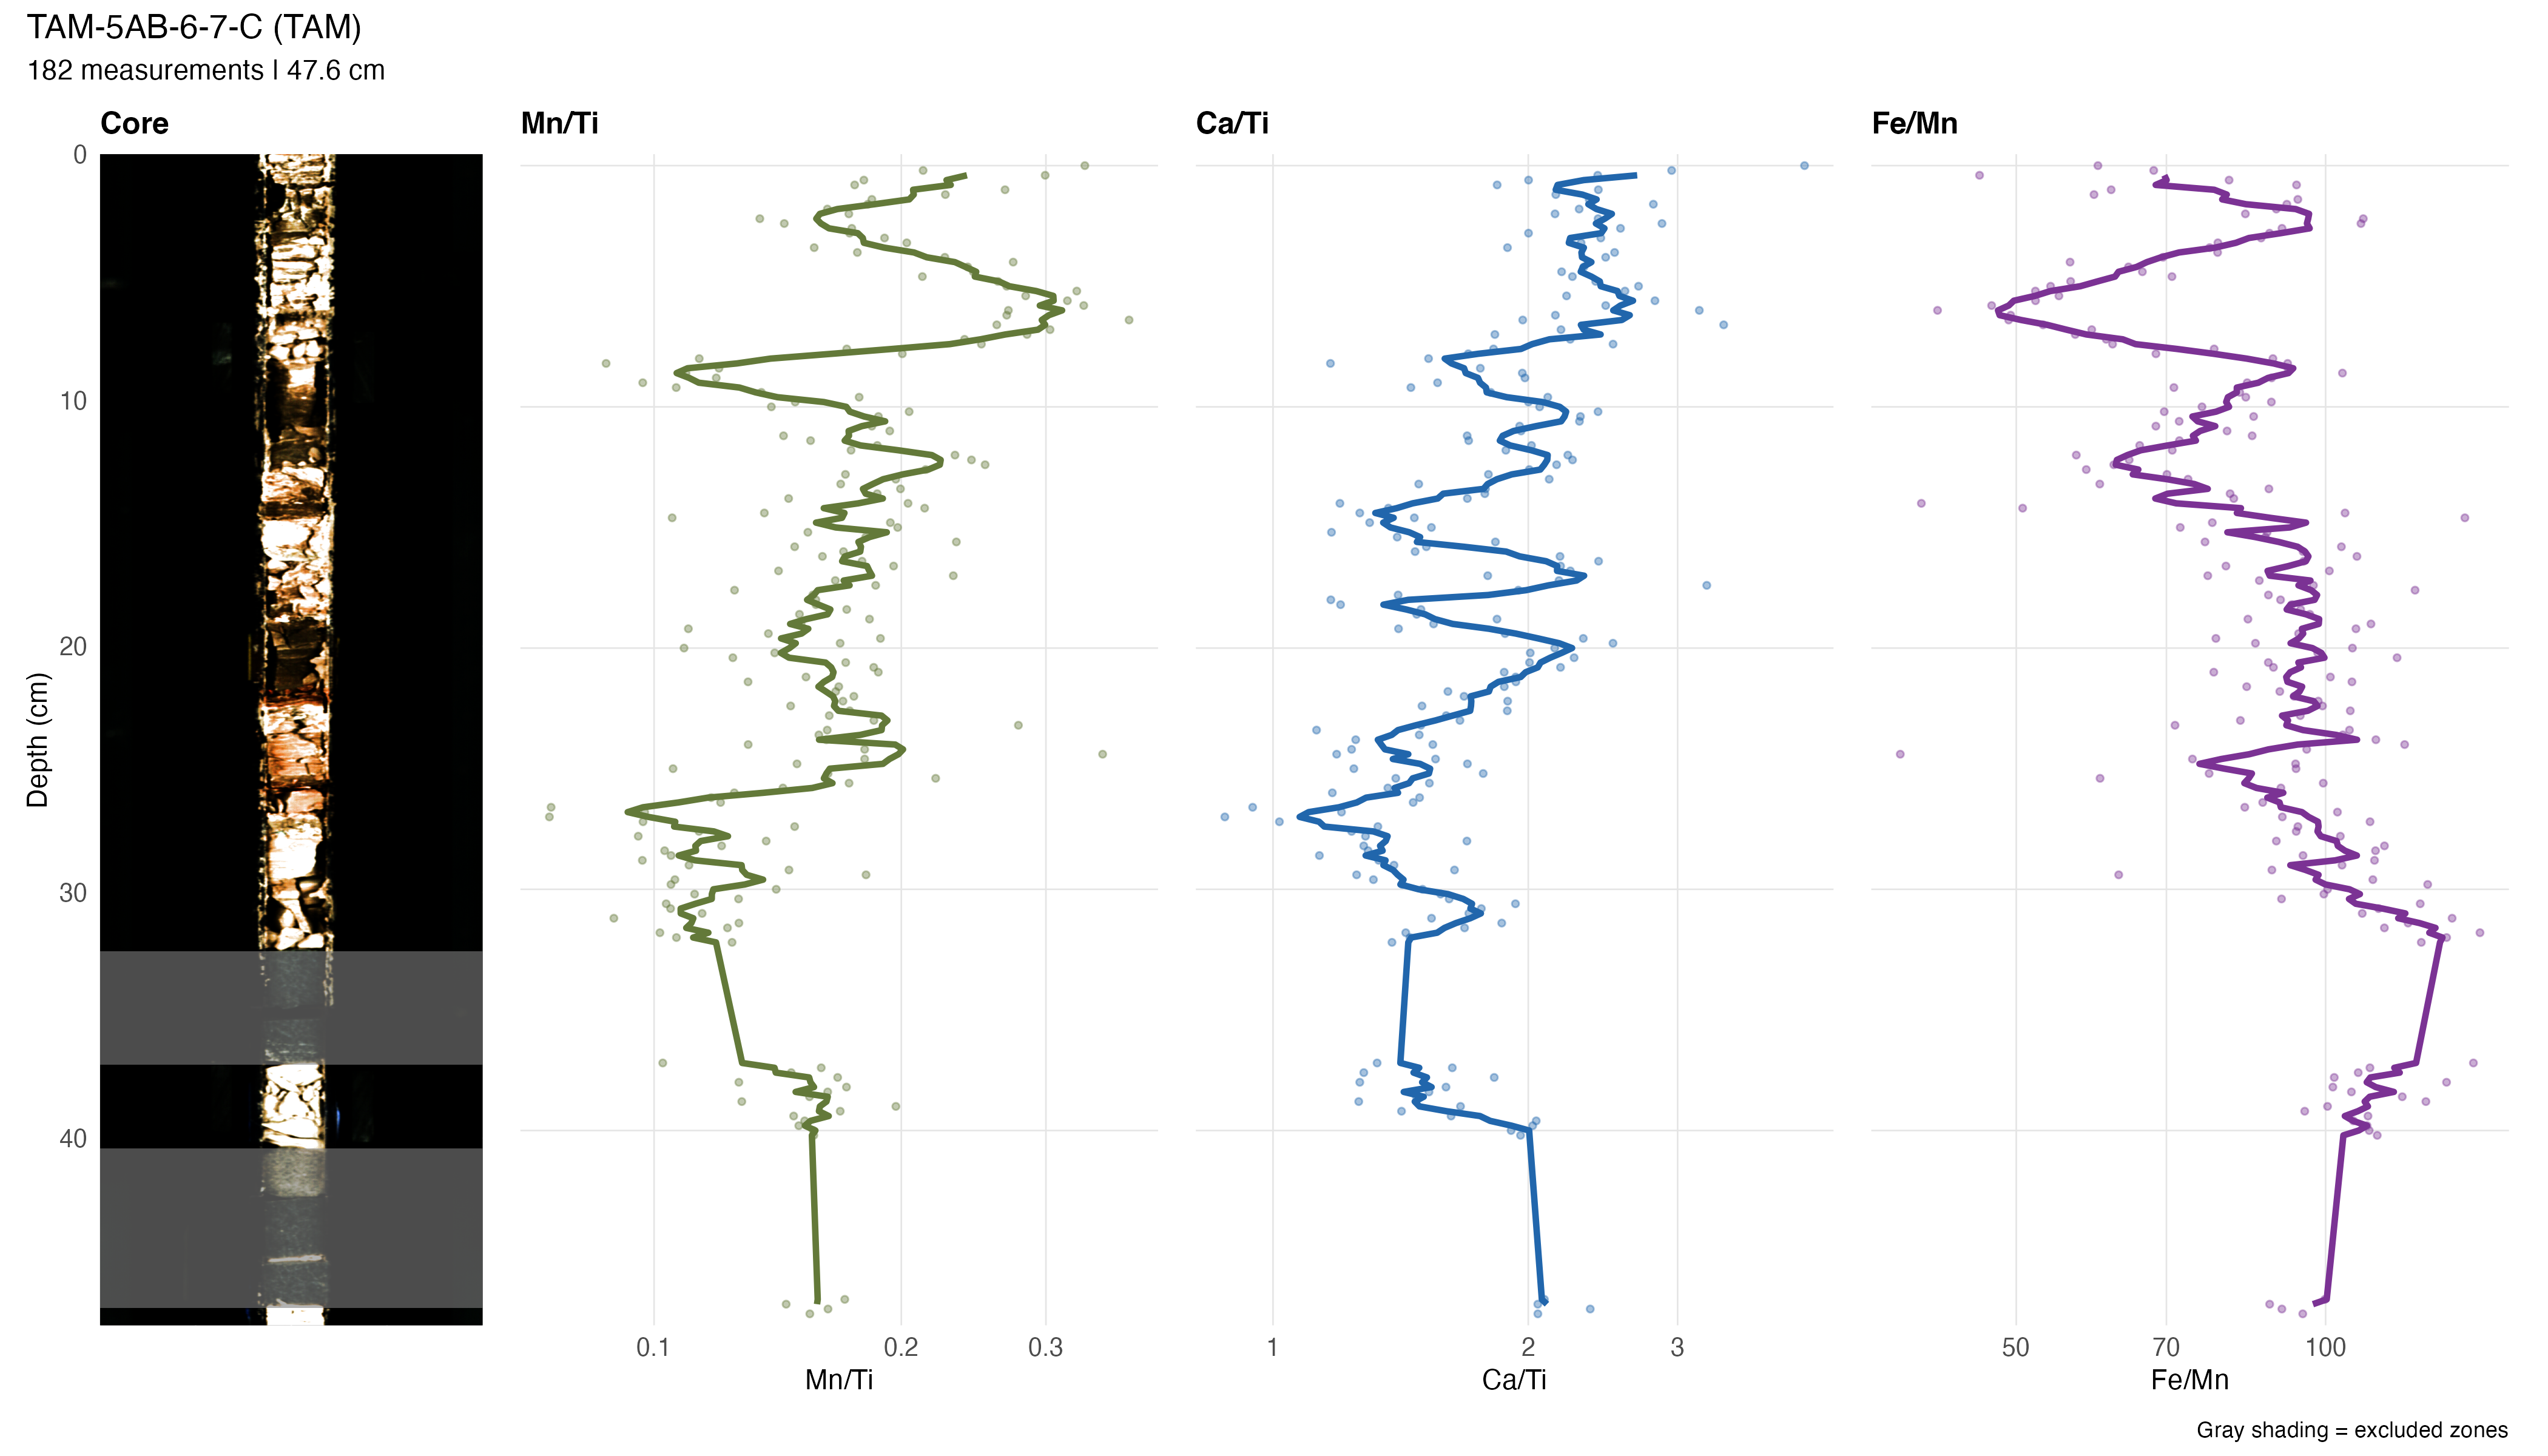
\includegraphics[width=\textwidth]{../output/figures/temporal_overlap/top_TAM-5AB-6-7-C.png}
    \caption{TAM-5AB-6-7-C: Youngest TAM section ($\sim$12.9 Ma). Core image with Mn/Ti, Ca/Ti, and Fe/Mn profiles. This section shows characteristic TAM dysoxic conditions (low Mn/Ti) with occasional carbonate-rich intervals (Ca/Ti peaks).}
    \label{fig:tam-top}
\end{figure}

\textbf{Key observations}:
\begin{itemize}
    \item Persistently low Mn/Ti indicates sustained bottom-water dysoxia
    \item Ca/Ti peaks correlate with visible lighter (shell-rich) horizons
    \item Fe/Mn remains elevated, confirming reducing conditions
\end{itemize}

\subsection{TAM Core Top Continuation: TAM-5AB-6-7-B-RUN2}

\begin{figure}[H]
    \centering
    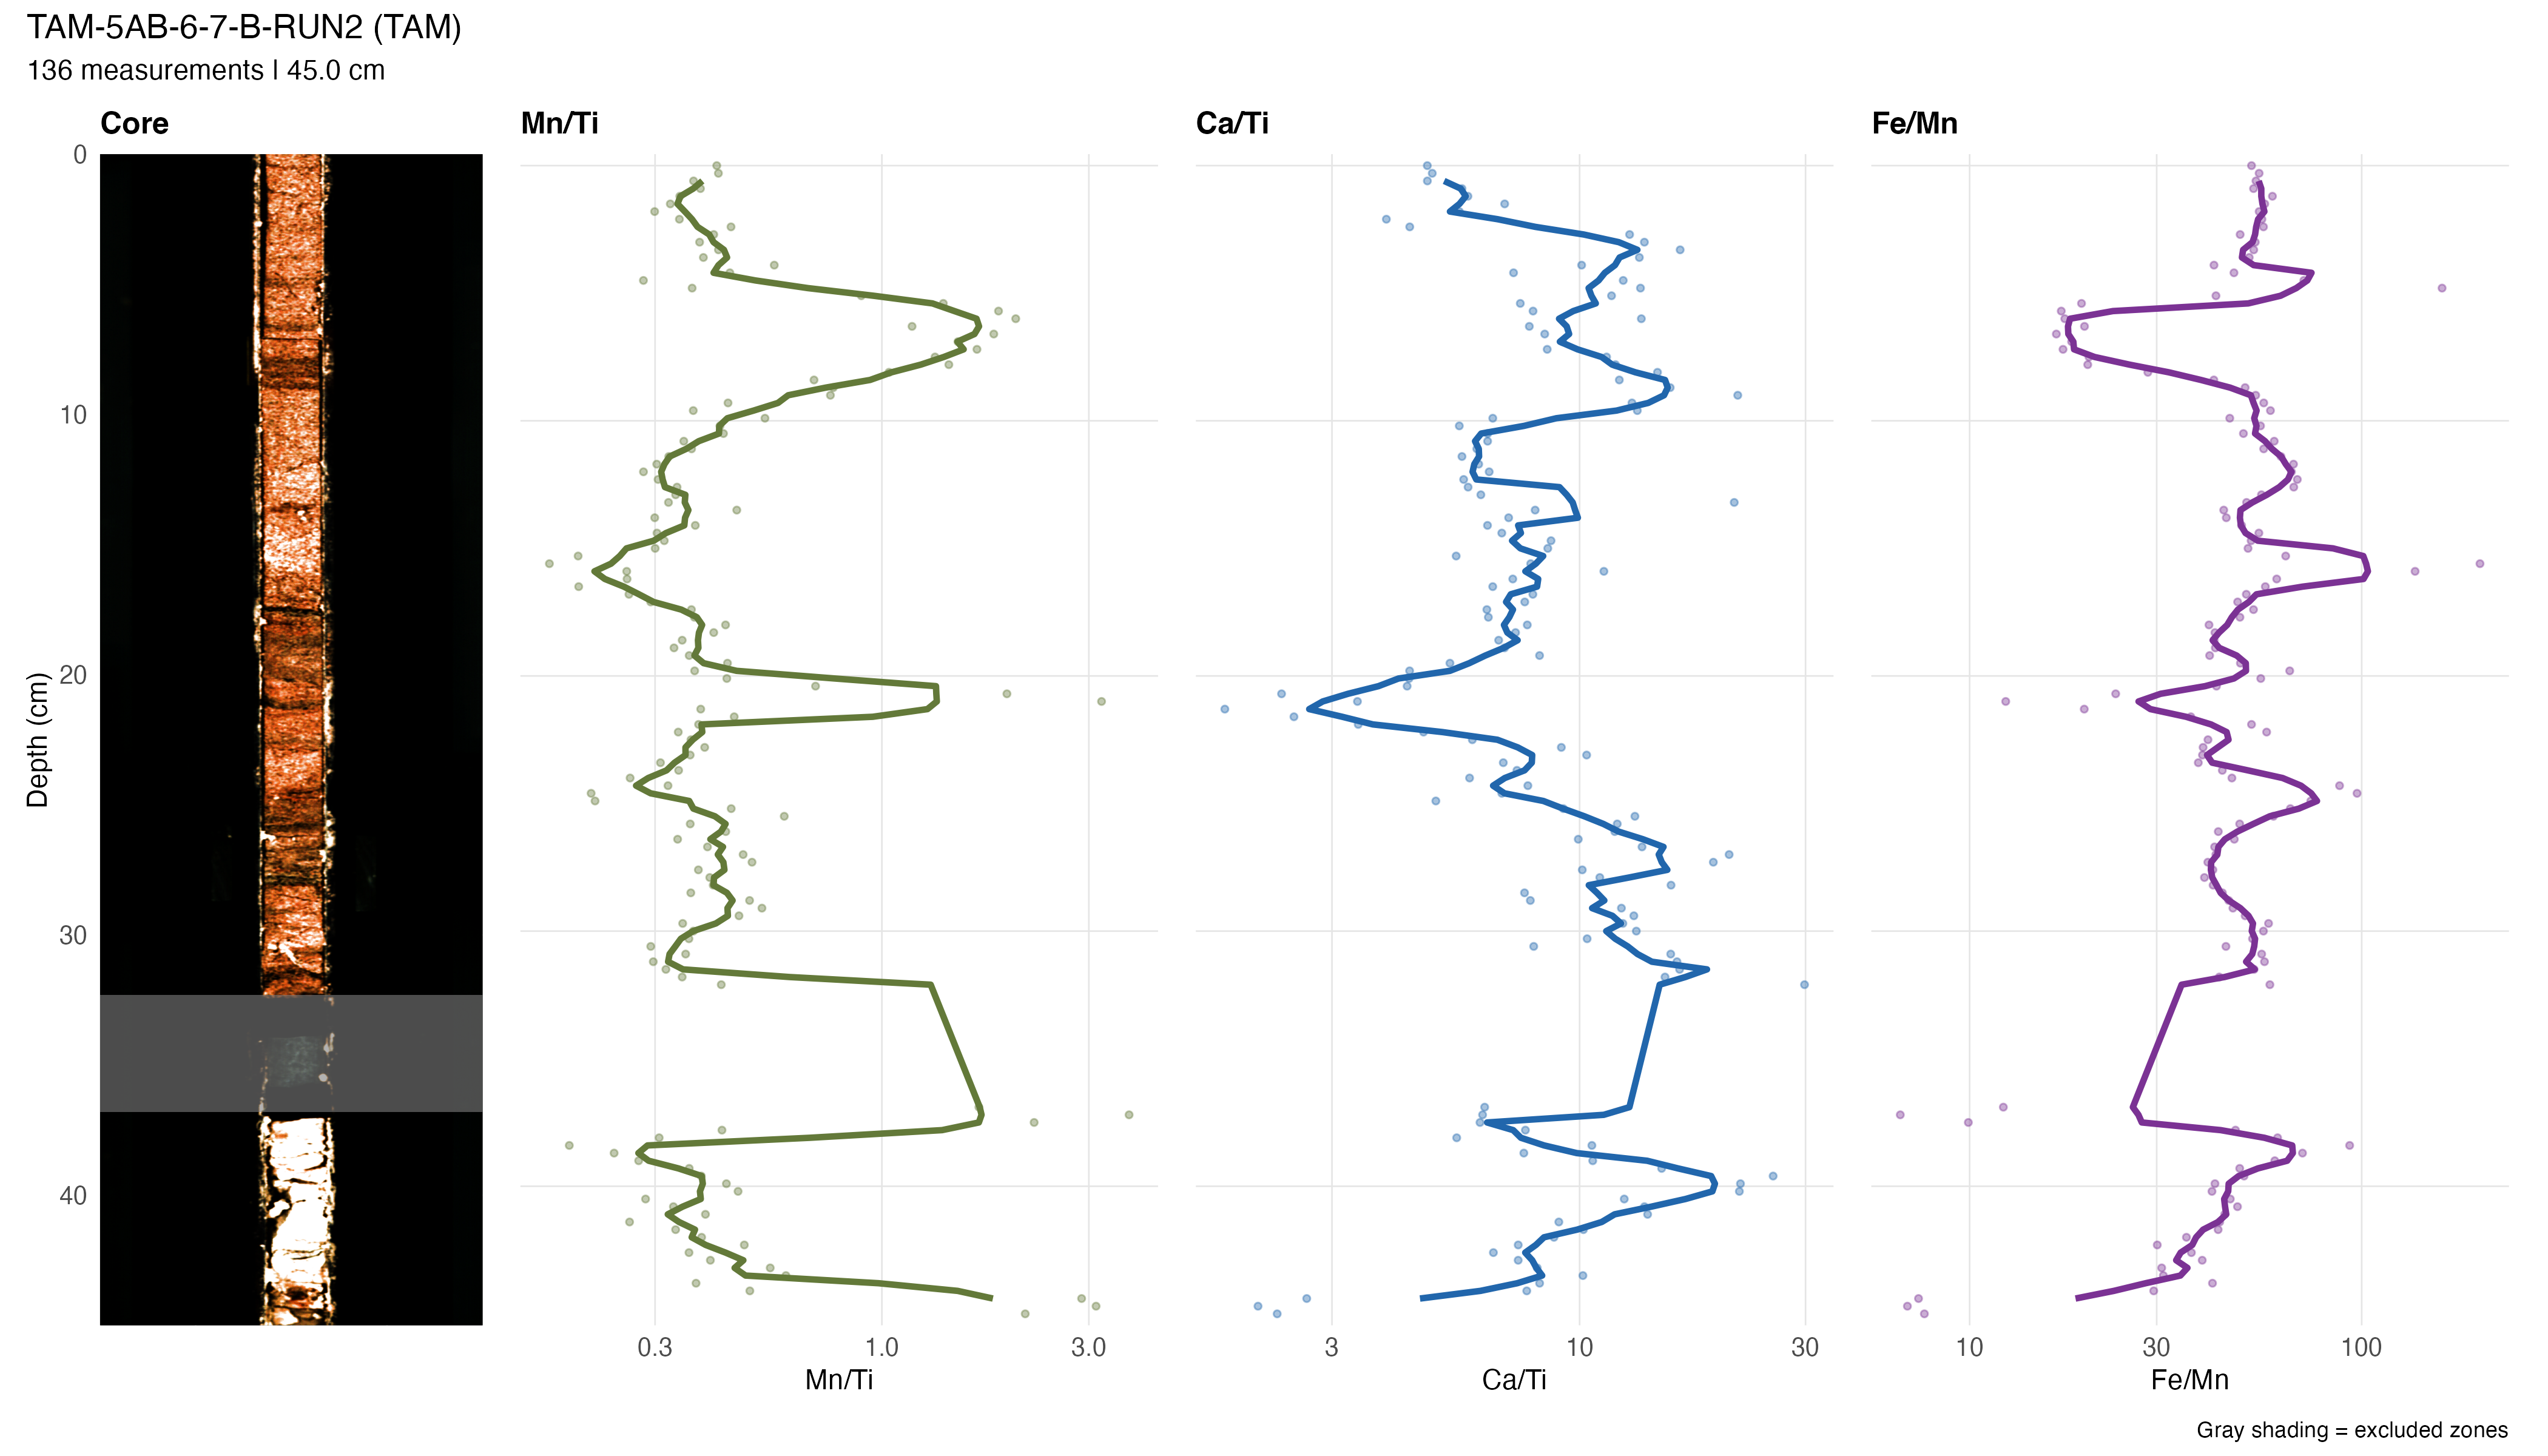
\includegraphics[width=\textwidth]{../output/figures/temporal_overlap/top_TAM-5AB-6-7-B-RUN2.png}
    \caption{TAM-5AB-6-7-B-RUN2: Continuation of youngest TAM sequence. Similar proxy patterns confirm consistent environmental conditions through this interval.}
    \label{fig:tam-top-b}
\end{figure}

\subsection{SC Core Top: SC8-A ($\sim$13.3 Ma)}

The youngest SC section represents the most recent SC deposits, roughly 400 kyr older than the TAM top.

\begin{figure}[H]
    \centering
    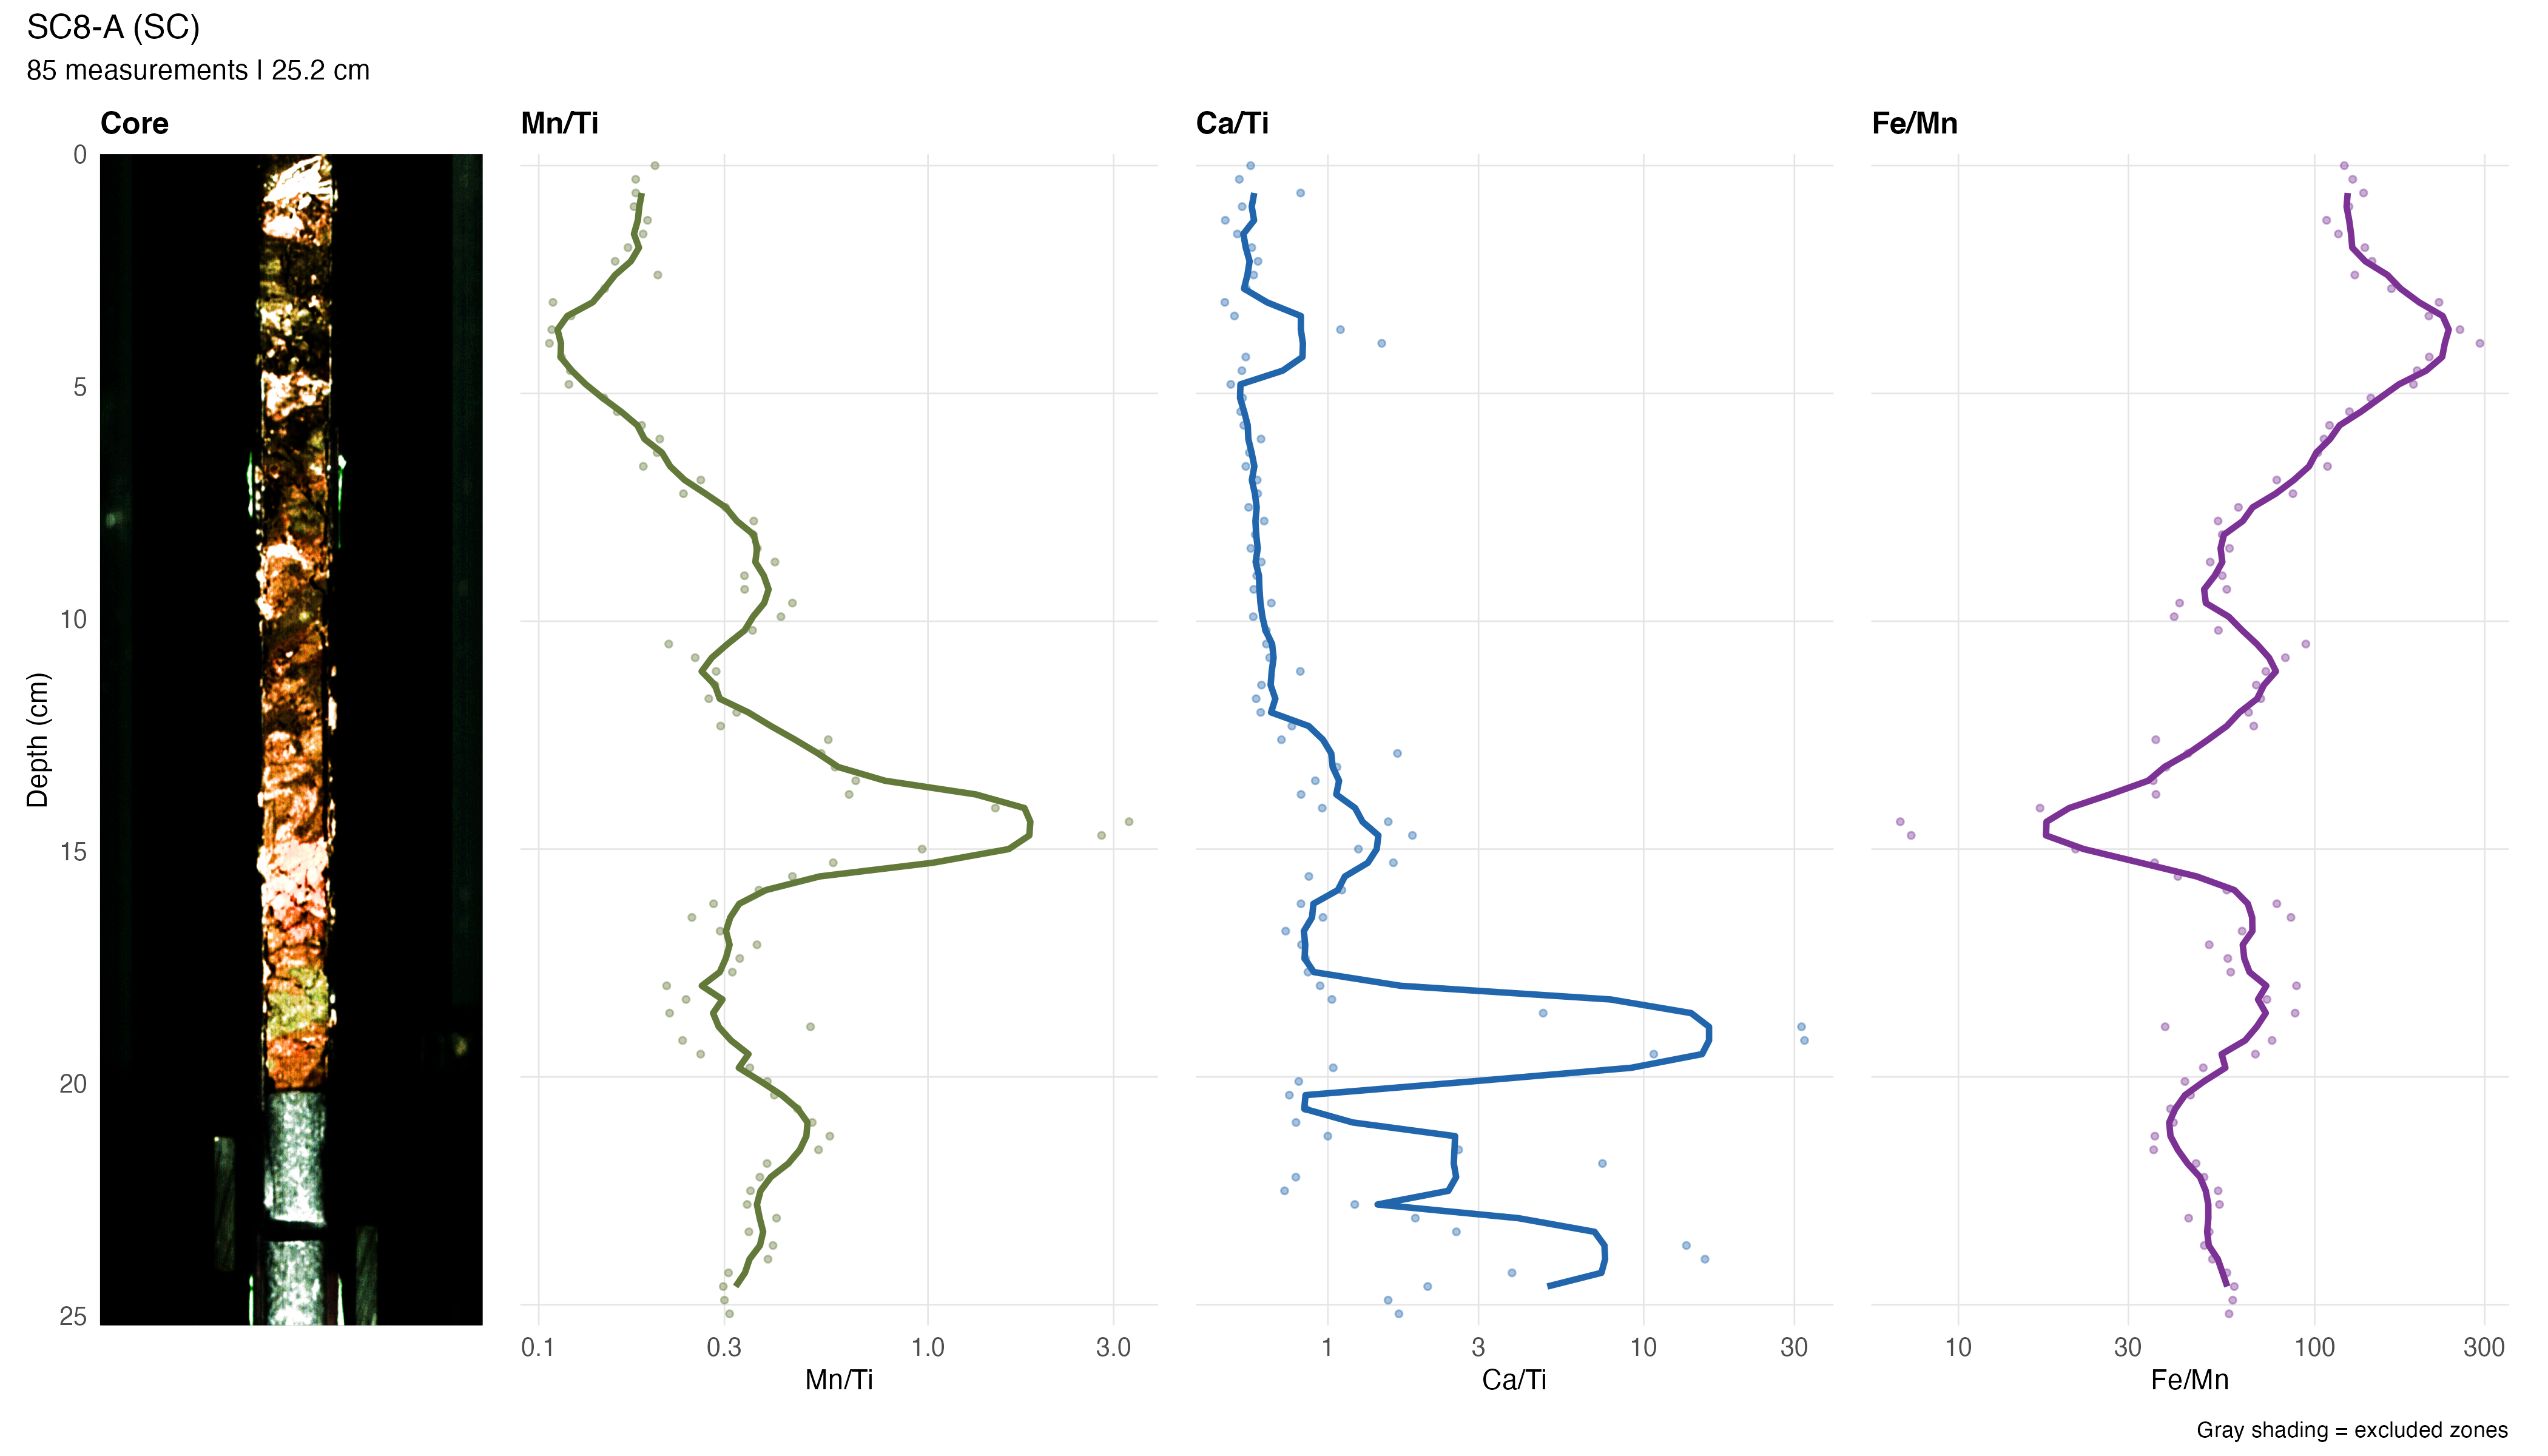
\includegraphics[width=\textwidth]{../output/figures/temporal_overlap/fig4_SC8-A.png}
    \caption{SC8-A: Youngest SC section ($\sim$13.3 Ma). Note the notably higher Mn/Ti values compared to TAM, indicating more oxic bottom-water conditions at SC. This section falls within the temporal overlap with TAM.}
    \label{fig:sc-top}
\end{figure}

\textbf{Key observations}:
\begin{itemize}
    \item Higher Mn/Ti than TAM indicates better-oxygenated conditions
    \item More variable proxy signals suggest dynamic, ventilated environment
    \item Ca/Ti generally lower than TAM, reflecting different carbonate input
\end{itemize}

\subsection{Top of Cores Comparison}

\begin{figure}[H]
    \centering
    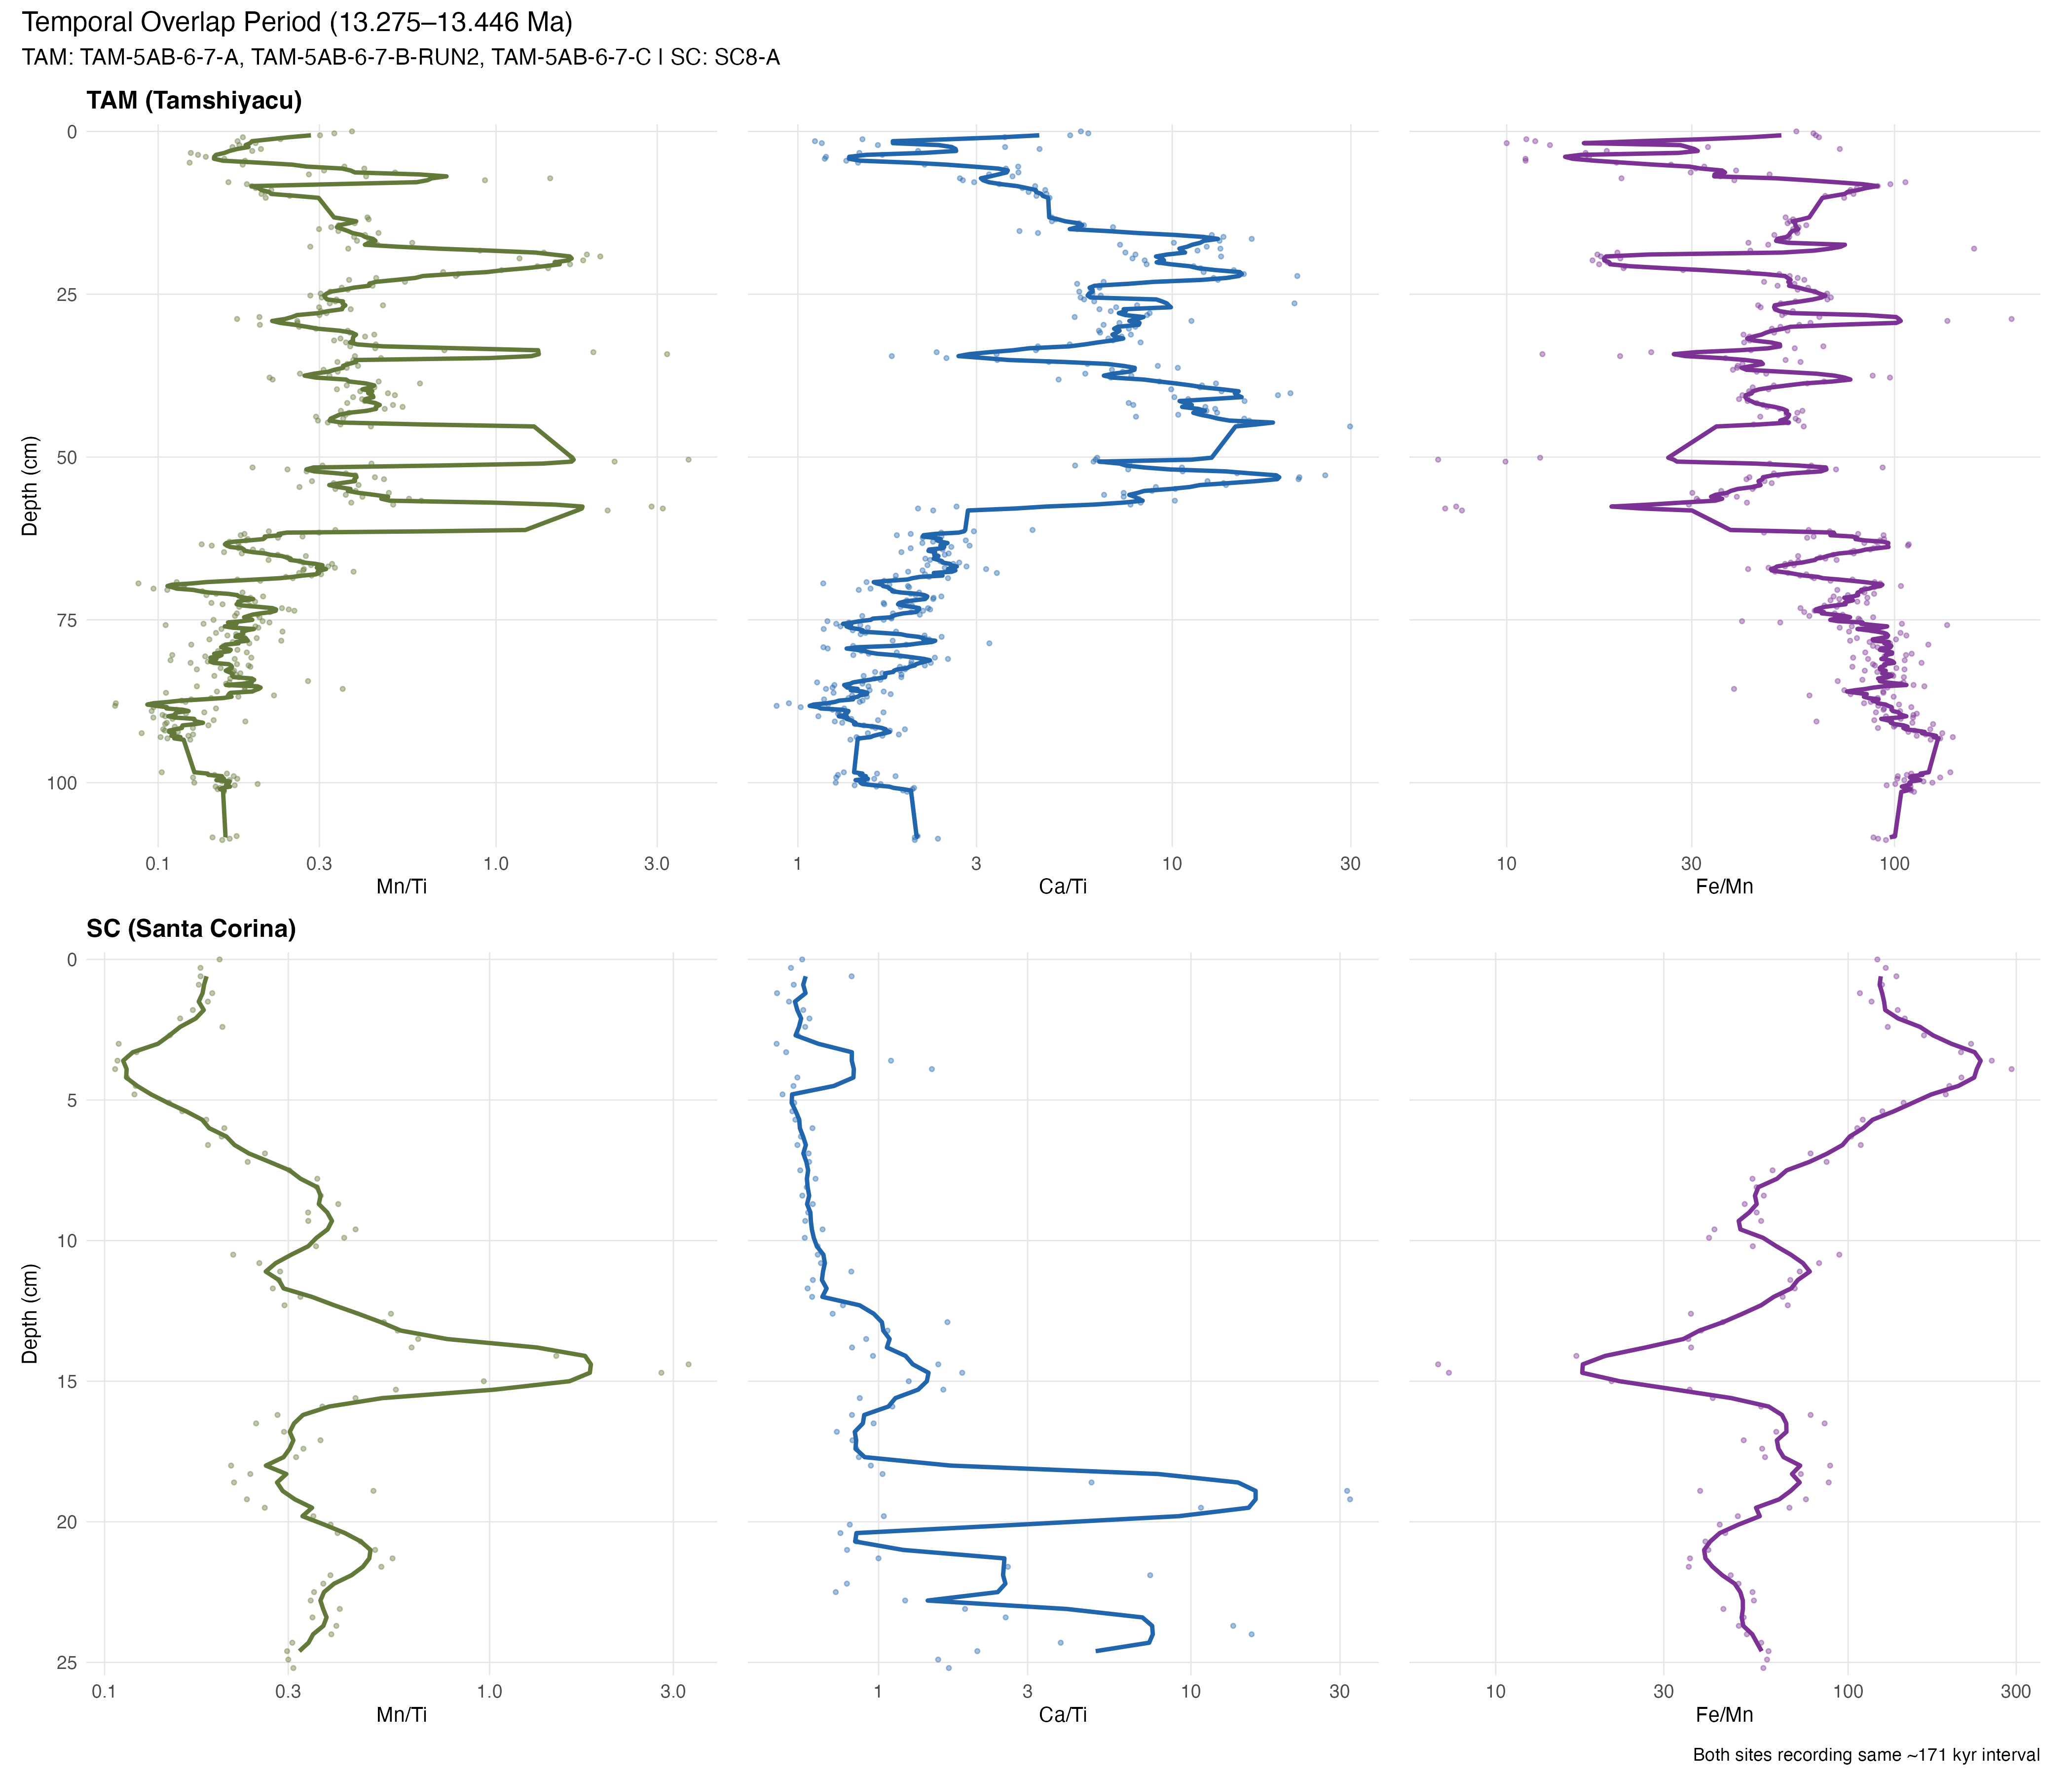
\includegraphics[width=\textwidth]{../output/figures/temporal_overlap/top_cores_comparison.png}
    \caption{Direct comparison of youngest sections from both cores. Top: TAM GROUP3 (TAM-5AB-6-7 sections, $\sim$12.9 Ma). Bottom: SC8-A ($\sim$13.3 Ma). Despite being $\sim$400 kyr apart, the fundamental site contrast (TAM dysoxic, SC oxic) is evident.}
    \label{fig:top-comparison}
\end{figure}

\begin{tcolorbox}[colback=yellow!10, colframe=orange!50!black, title=Site Contrast Summary]
\textbf{TAM (younger, distal lacustrine):} Low Mn/Ti (median 0.18), high Ca/Ti, persistent dysoxia\\
\textbf{SC (older, fluvio-lacustrine):} High Mn/Ti (median 0.37), variable proxies, better ventilated
\end{tcolorbox}

%==============================================================================
\section{Temporal Overlap Model}
%==============================================================================

The cores share a 171 kyr overlap period (13.275--13.446 Ma). Comparing these time-equivalent intervals tests whether site differences reflect spatial heterogeneity or temporal evolution.

\subsection{Age-Depth Framework}

\begin{figure}[H]
    \centering
    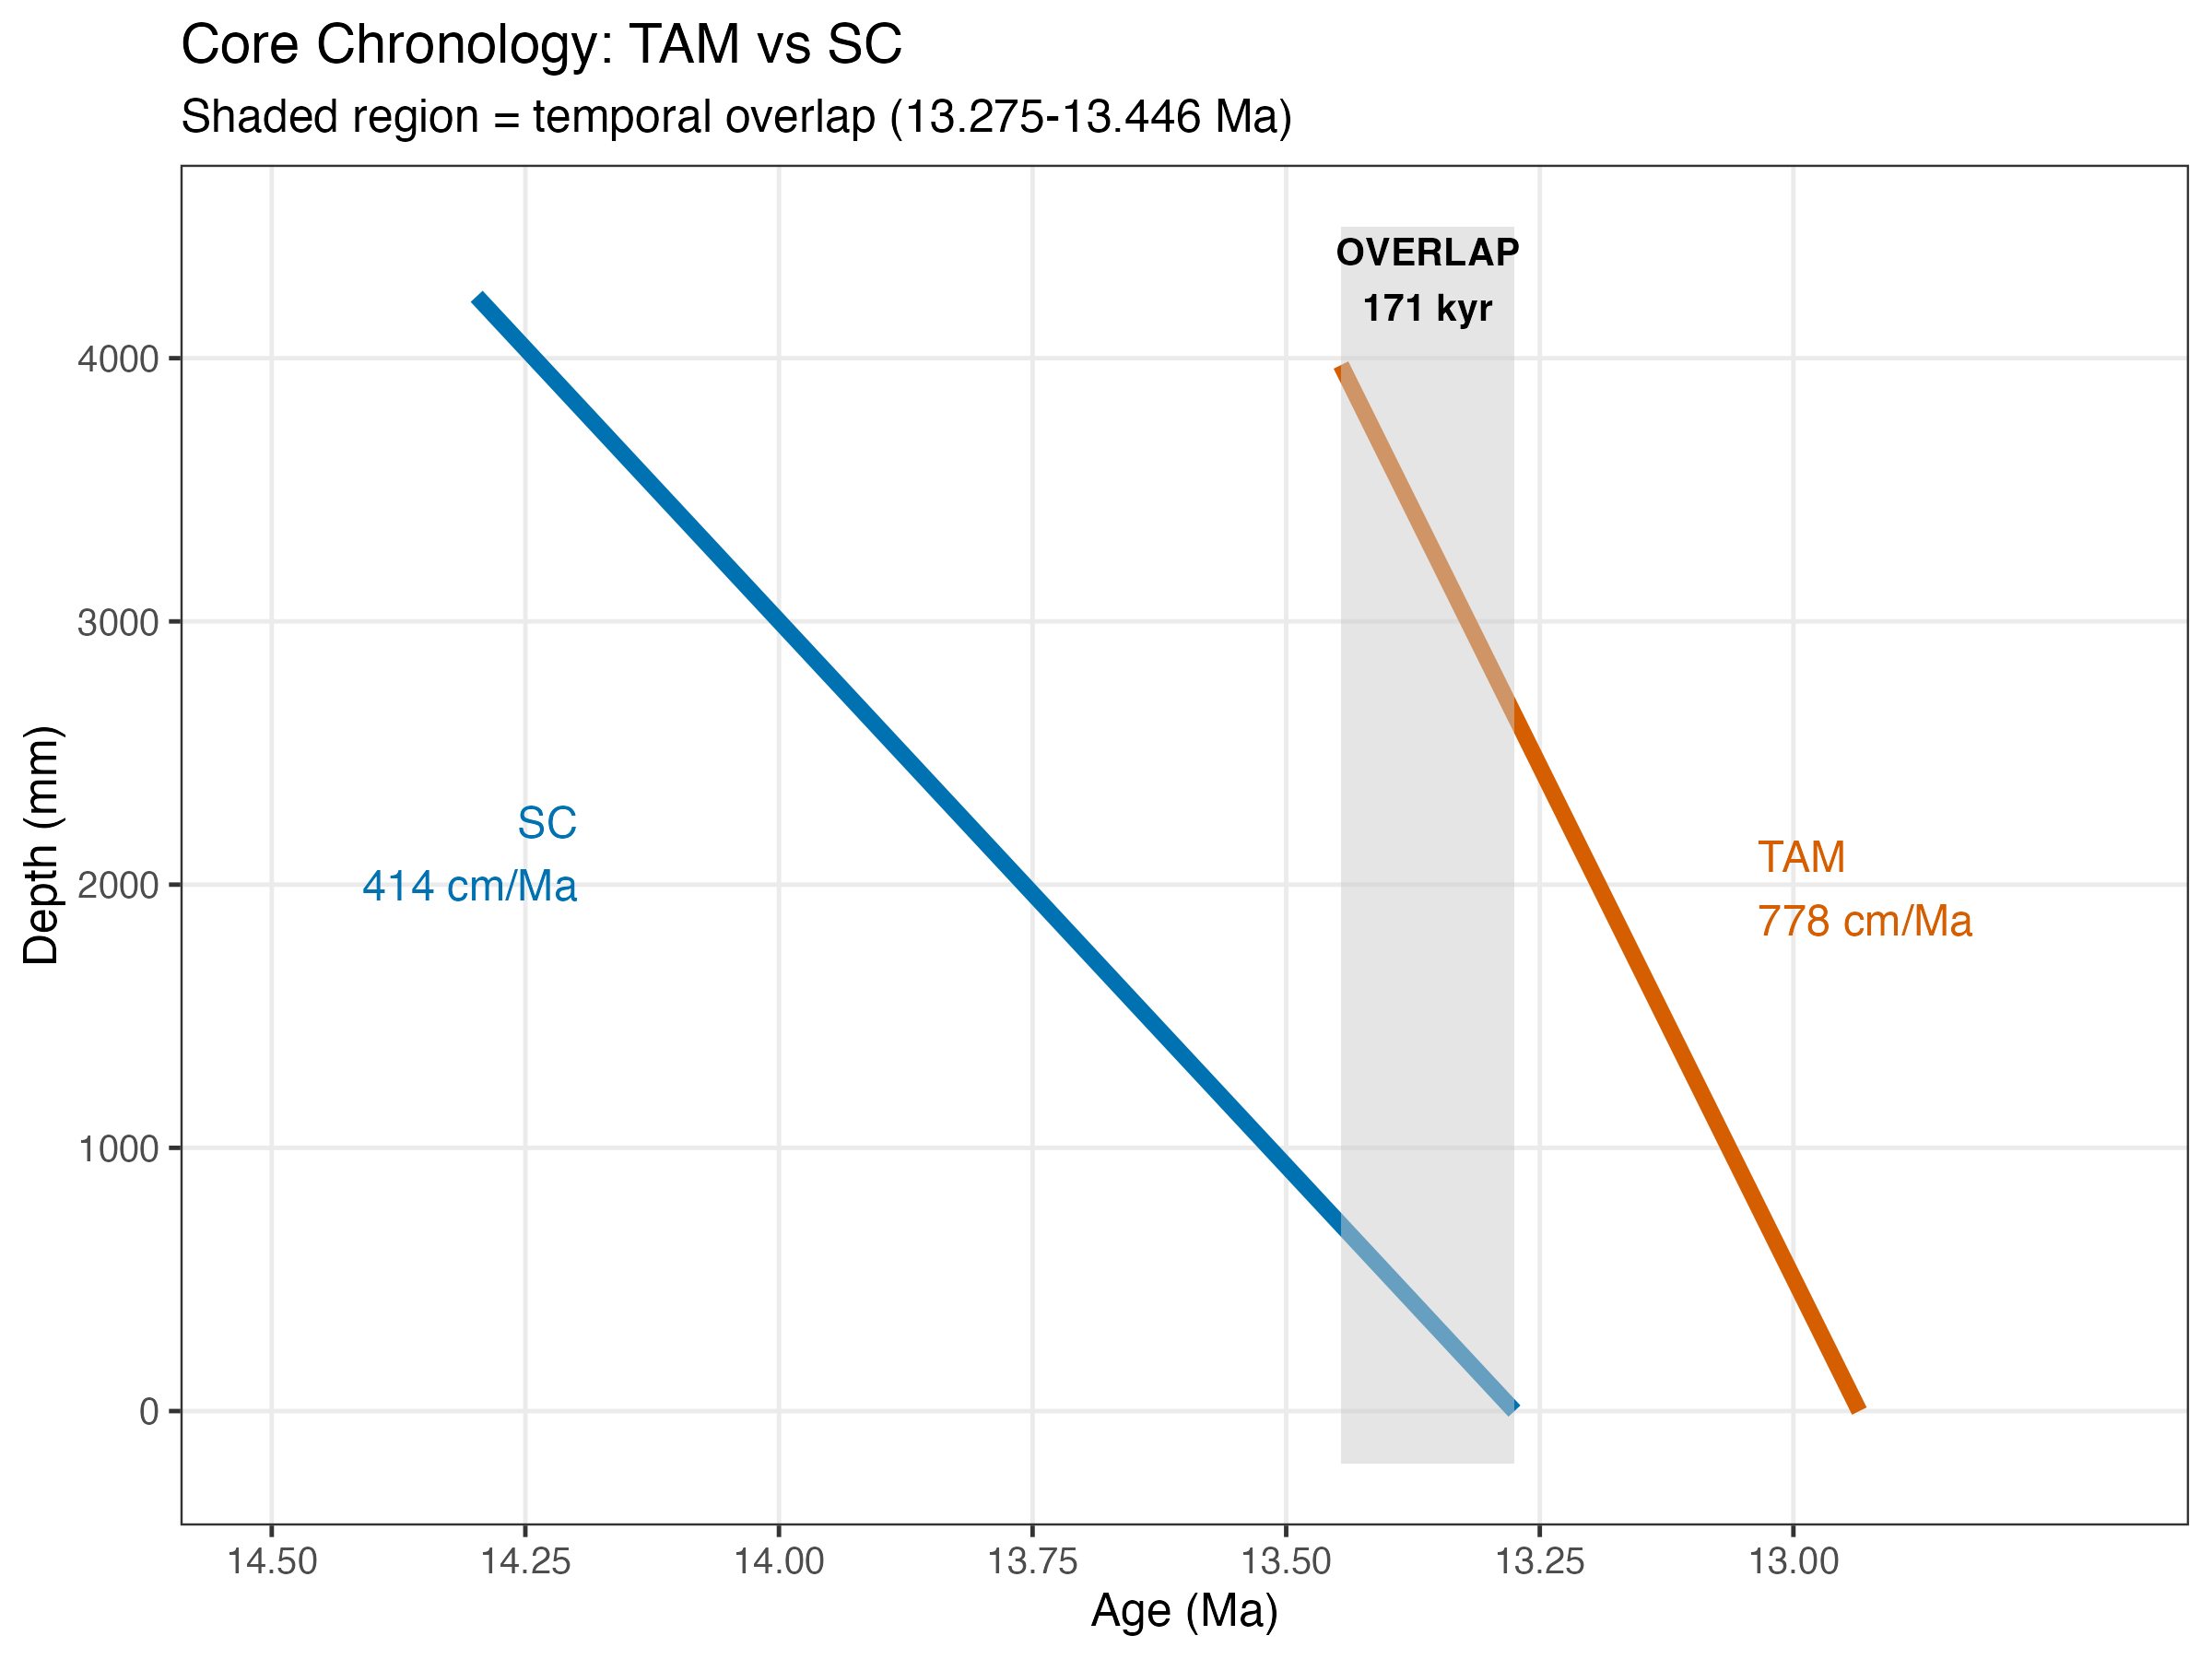
\includegraphics[width=0.9\textwidth]{../output/figures/temporal_overlap/fig2_age_depth_model.png}
    \caption{Age-depth model for TAM and SC cores. Yellow shading indicates the 171 kyr overlap period. TAM's higher sedimentation rate (778 cm/Ma) provides finer temporal resolution but shorter time coverage than SC (414 cm/Ma).}
    \label{fig:age-model}
\end{figure}

\subsection{TAM Overlap Sections (Bottom of TAM Core)}

The \textbf{oldest} TAM sections represent the overlap period. These are from the bottom of the TAM core.

\begin{figure}[H]
    \centering
    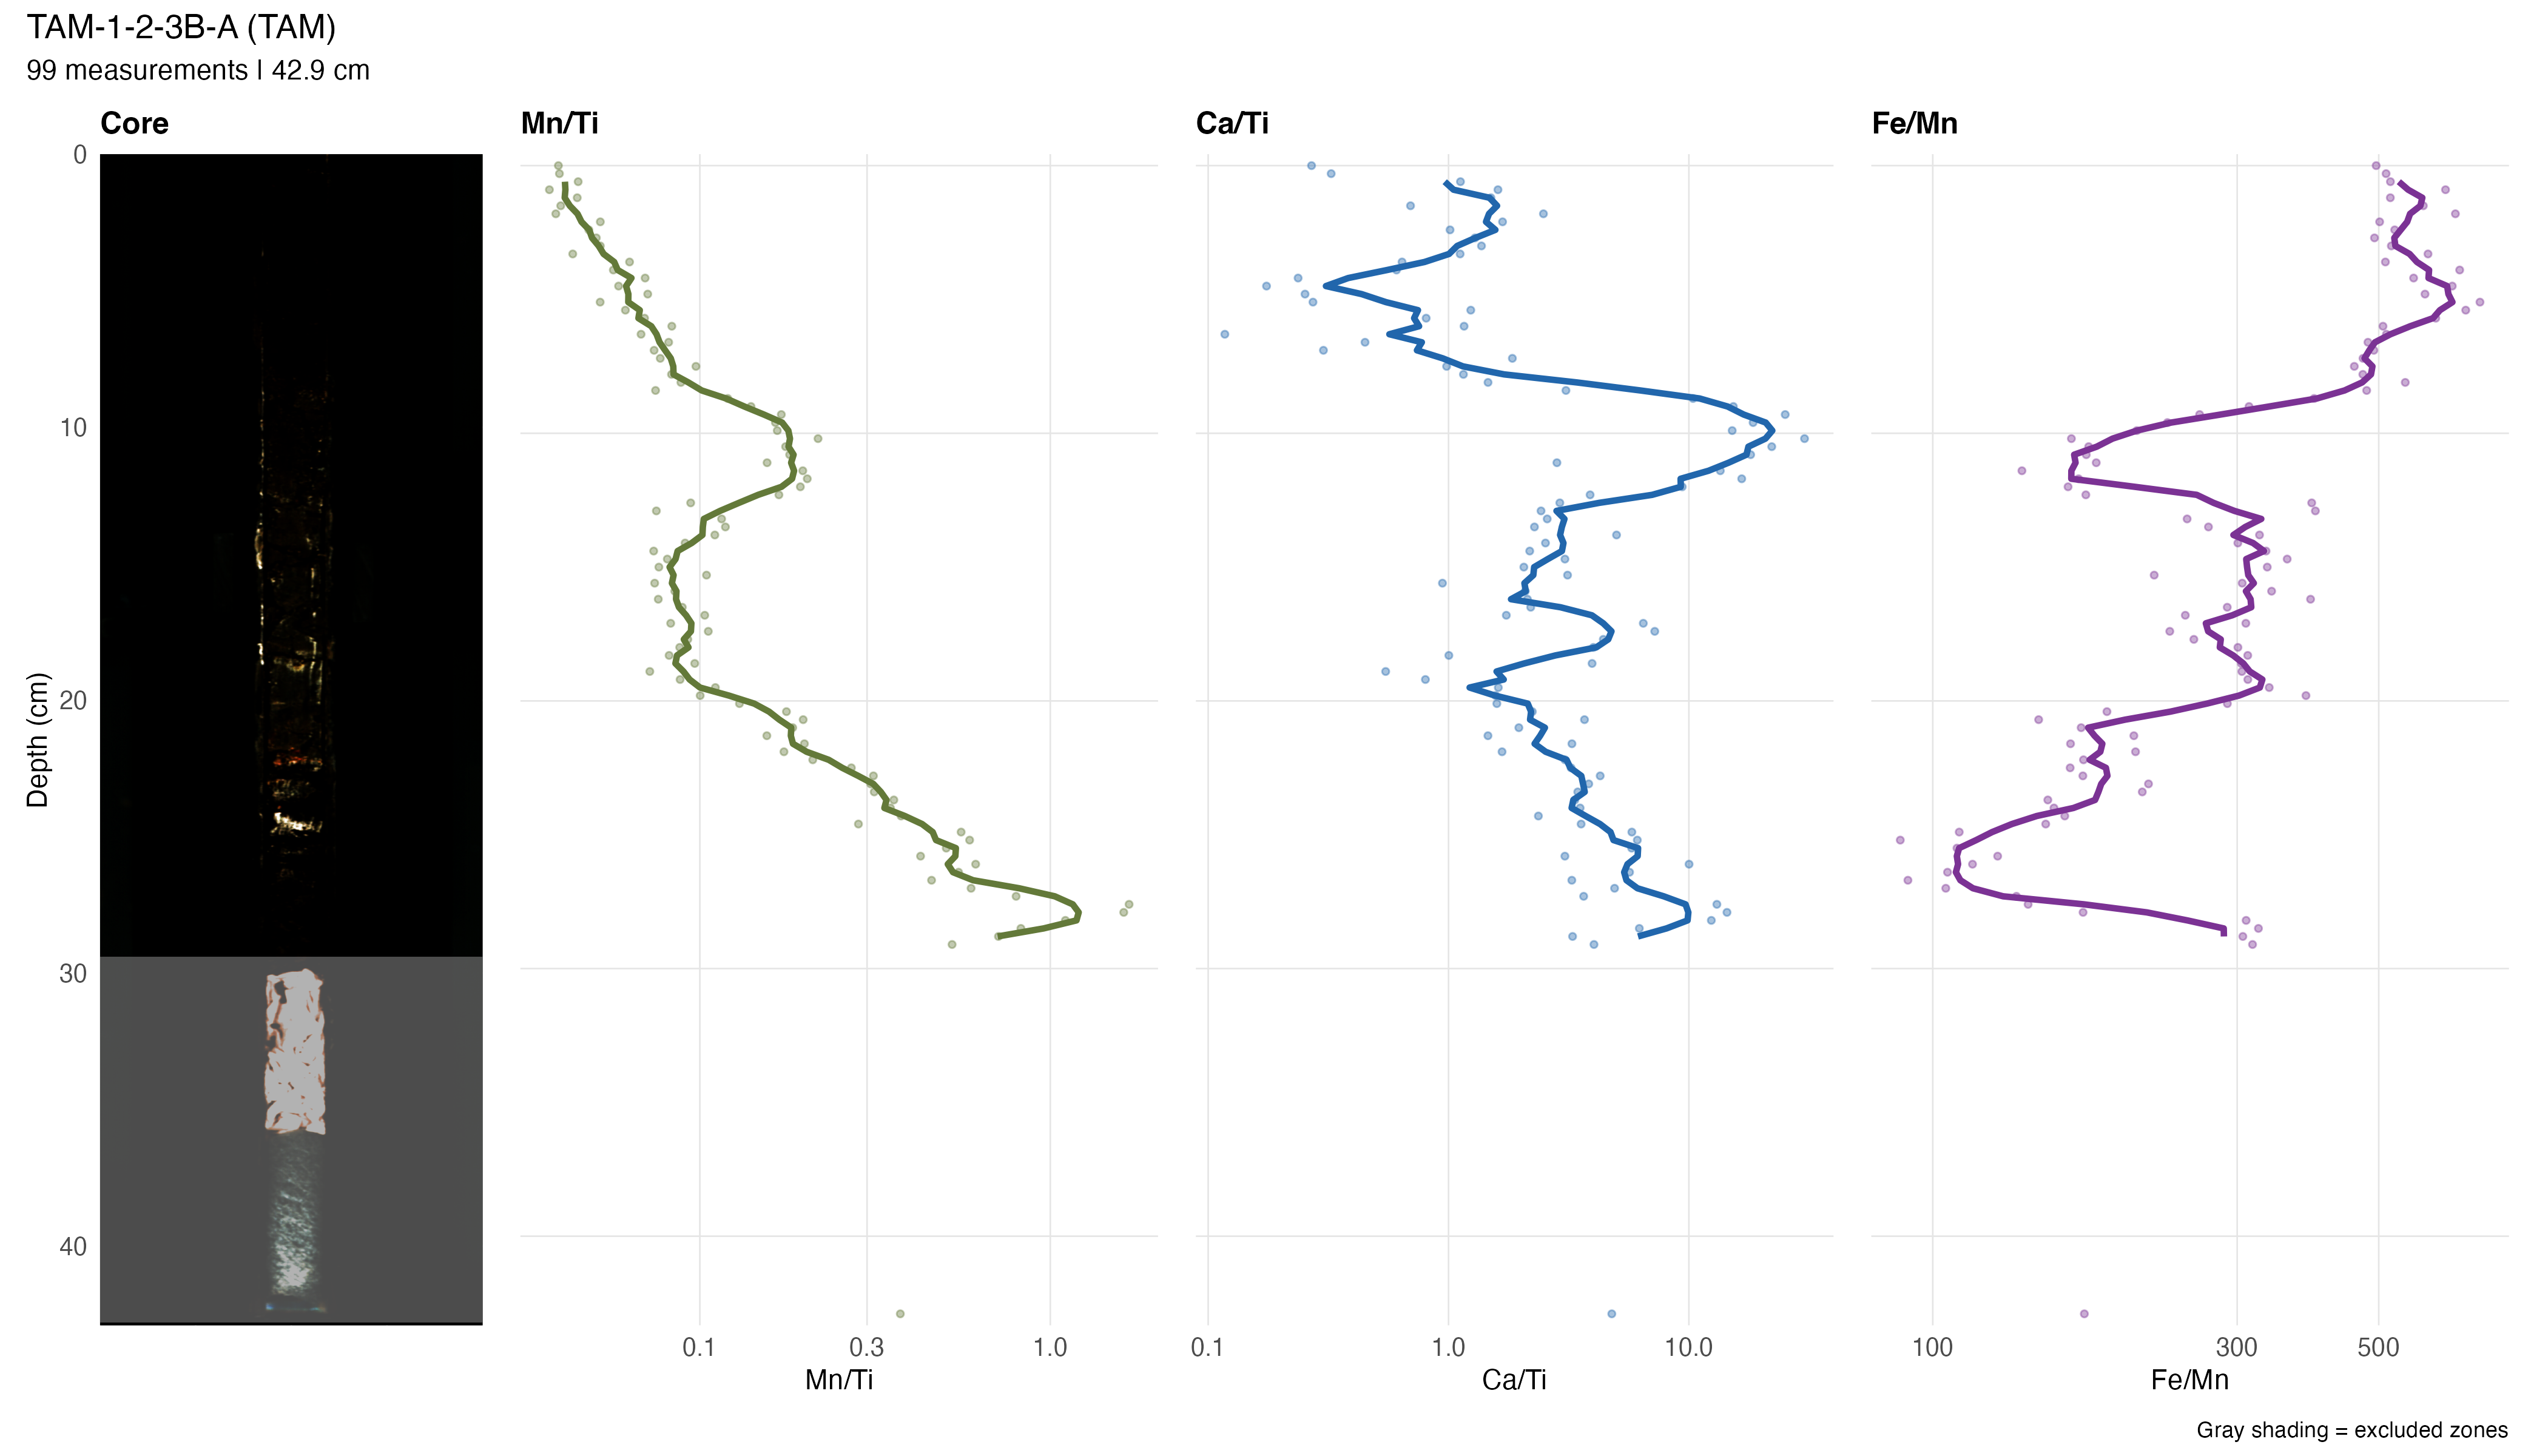
\includegraphics[width=\textwidth]{../output/figures/temporal_overlap/fig1_TAM-1-2-3B-A.png}
    \caption{TAM-1-2-3B-A: Oldest TAM section ($\sim$13.4 Ma), within the overlap period. Even at this oldest TAM level, Mn/Ti remains low, indicating the dysoxic signature is not simply a temporal trend but a persistent site characteristic.}
    \label{fig:tam-overlap-a}
\end{figure}

\begin{figure}[H]
    \centering
    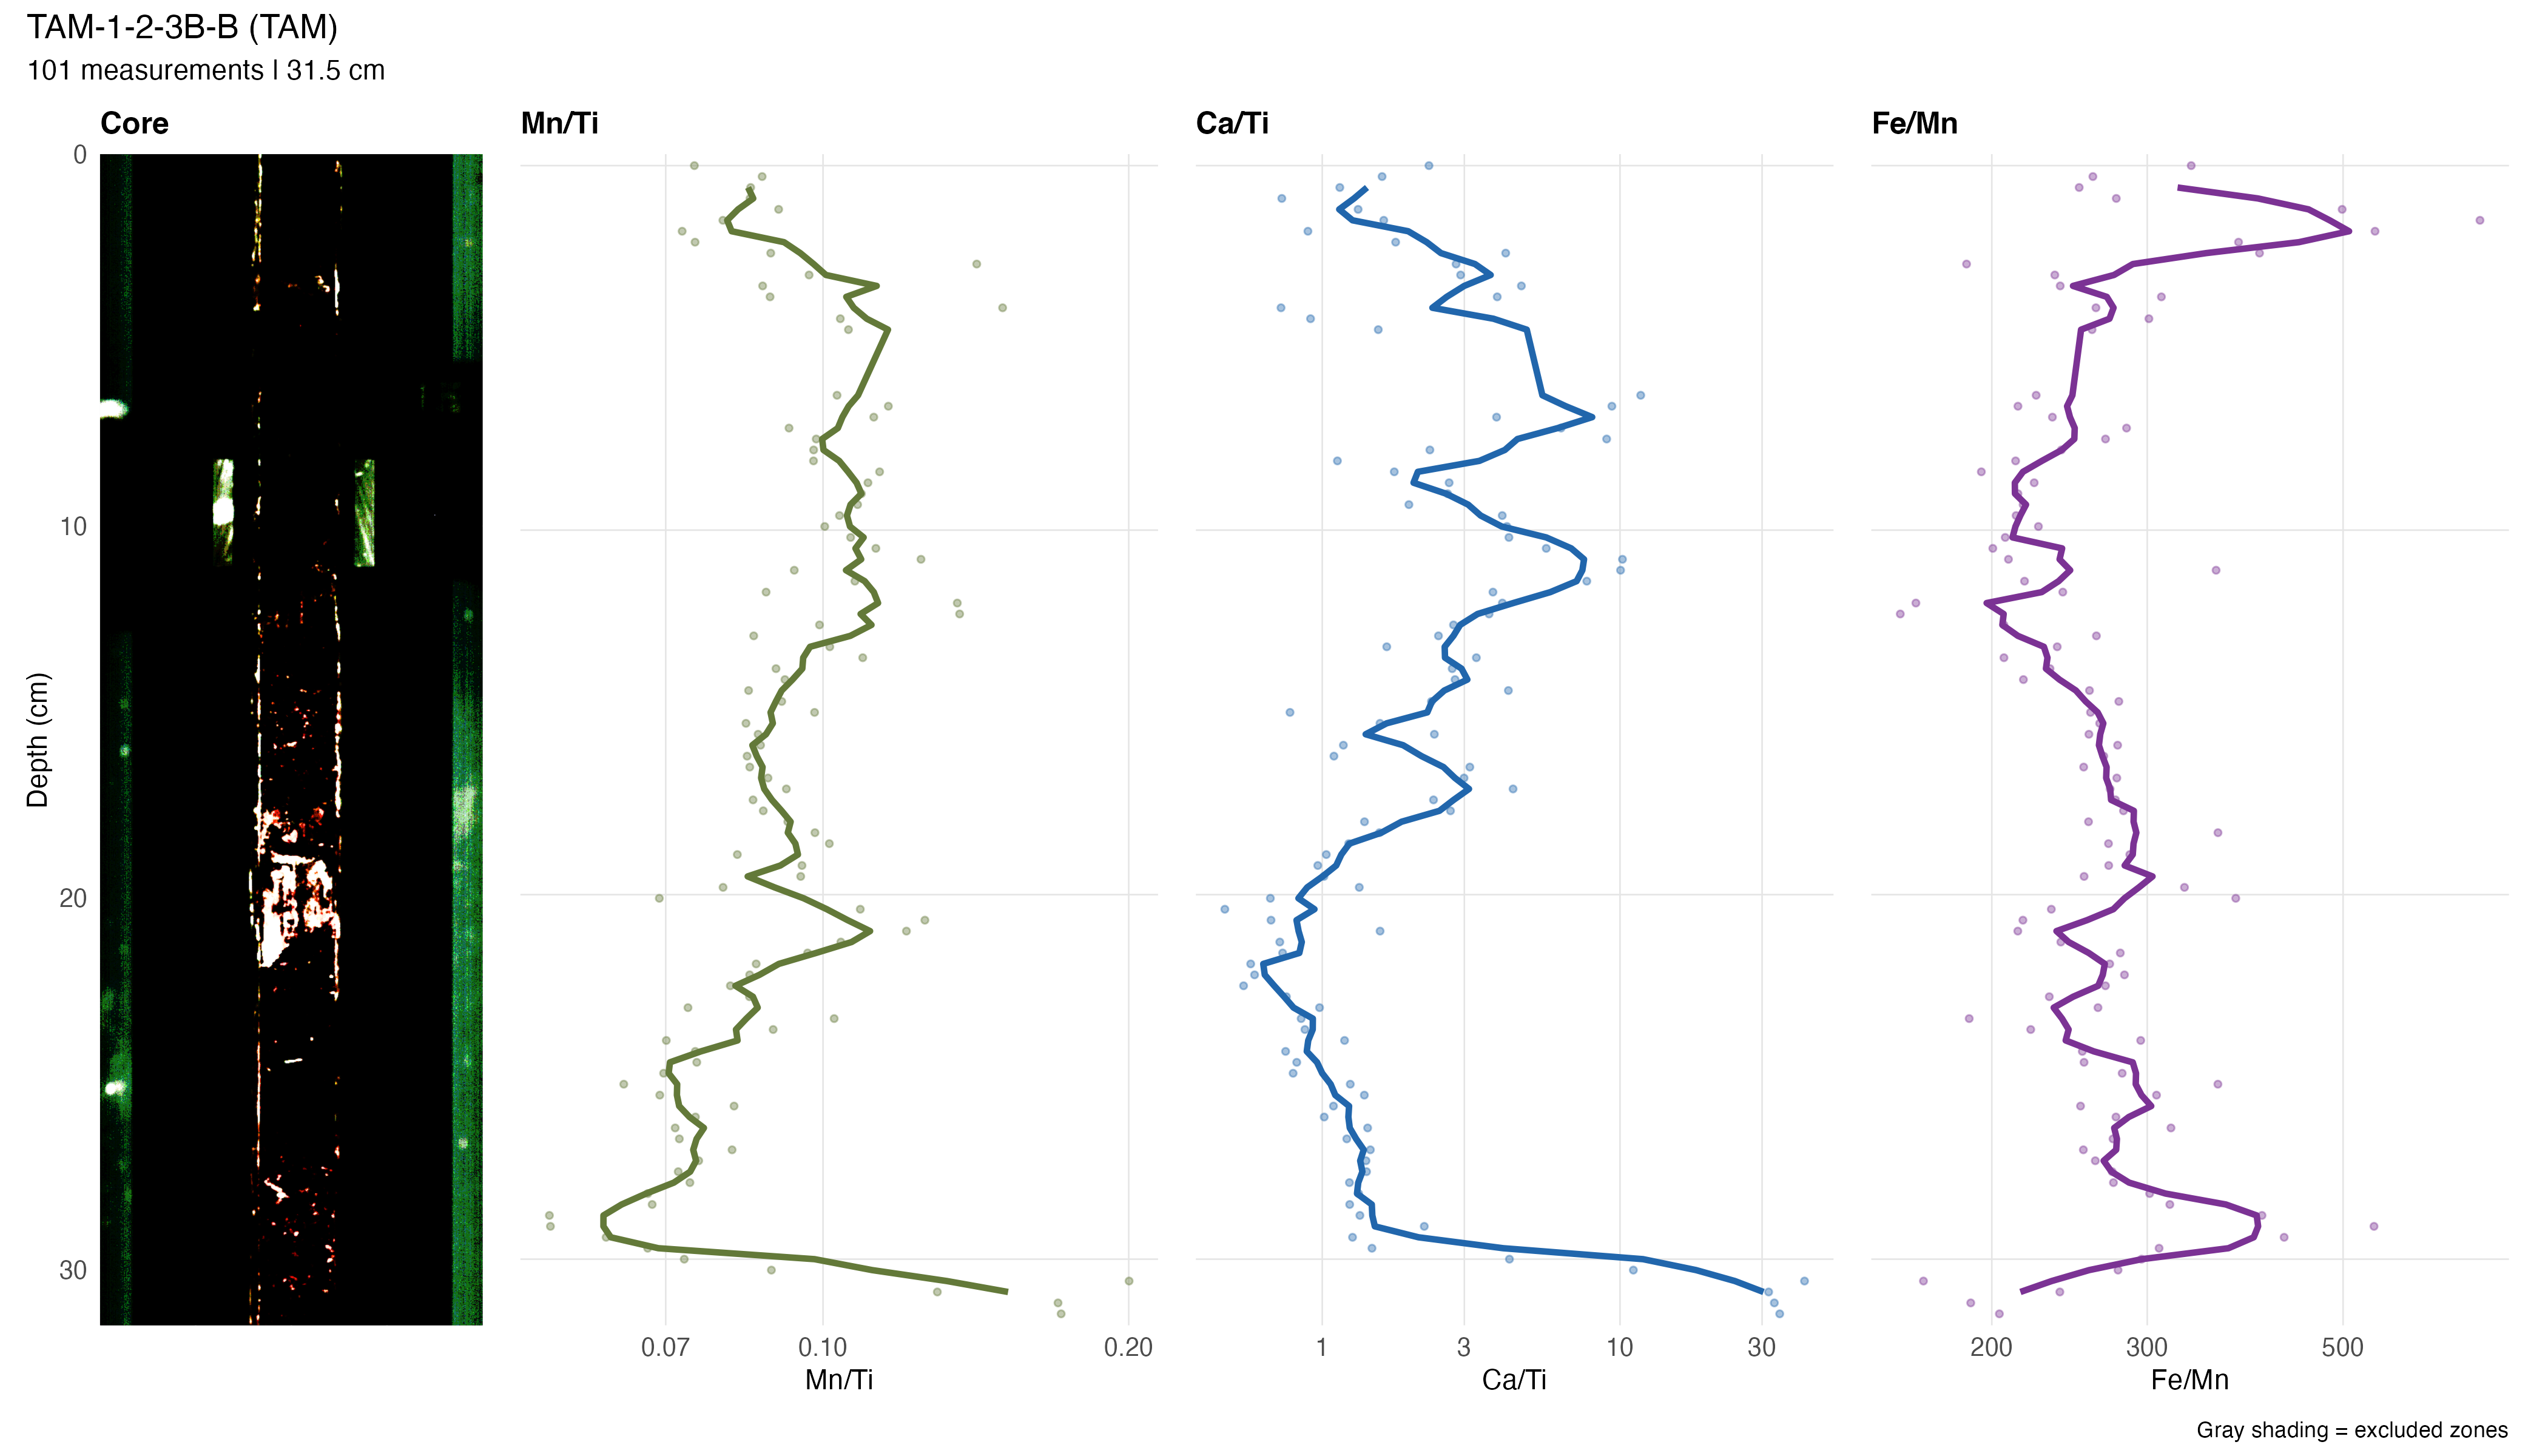
\includegraphics[width=\textwidth]{../output/figures/temporal_overlap/fig2_TAM-1-2-3B-B.png}
    \caption{TAM-1-2-3B-B: Continuation of oldest TAM sequence within the overlap period.}
    \label{fig:tam-overlap-b}
\end{figure}

\begin{figure}[H]
    \centering
    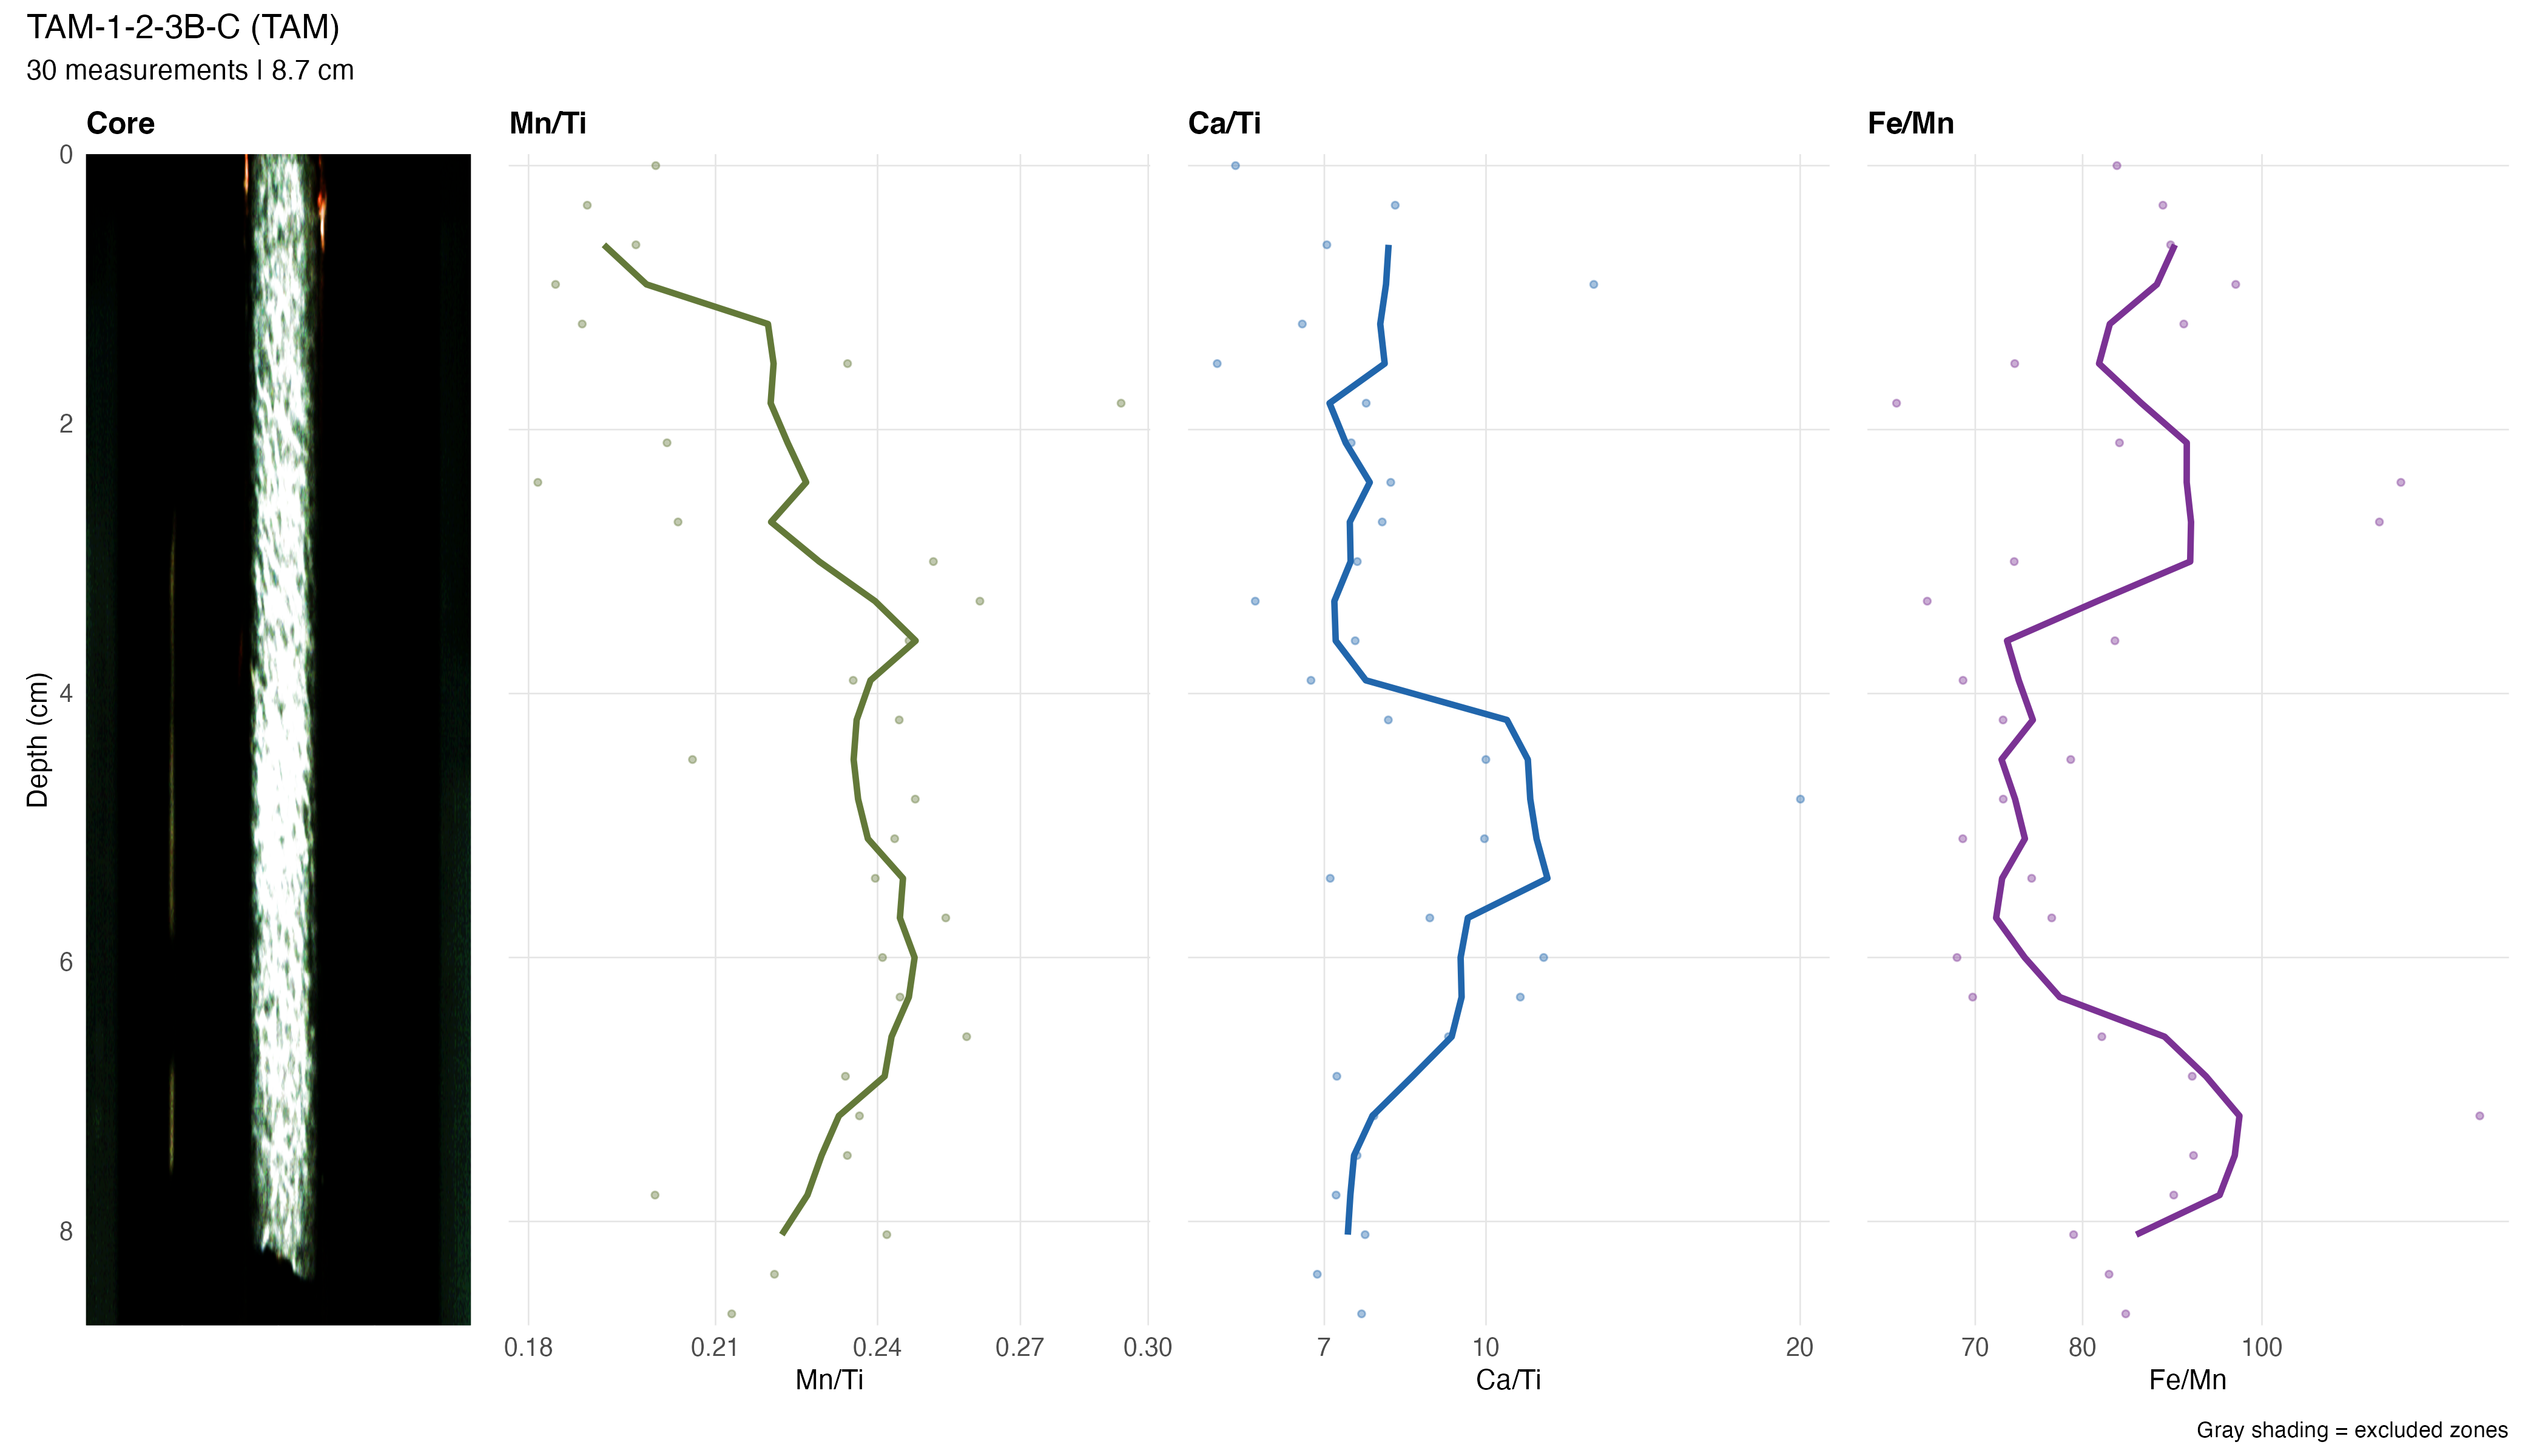
\includegraphics[width=\textwidth]{../output/figures/temporal_overlap/fig3_TAM-1-2-3B-C.png}
    \caption{TAM-1-2-3B-C: Upper portion of the TAM overlap interval. Small Mn/Ti excursions indicate brief oxygenation events punctuating the dysoxic baseline.}
    \label{fig:tam-overlap-c}
\end{figure}

\subsection{SC Overlap Section (Top of SC Core)}

SC8-A represents the SC overlap interval (shown above in Section 2.3). For the overlap comparison, we compare:
\begin{itemize}
    \item TAM: GROUP1 sections (TAM-1-2-3B-A, B, C) = bottom 133 cm
    \item SC: SC8-A section = top 71 cm
\end{itemize}

\subsection{Overlap Period Comparison}

\begin{figure}[H]
    \centering
    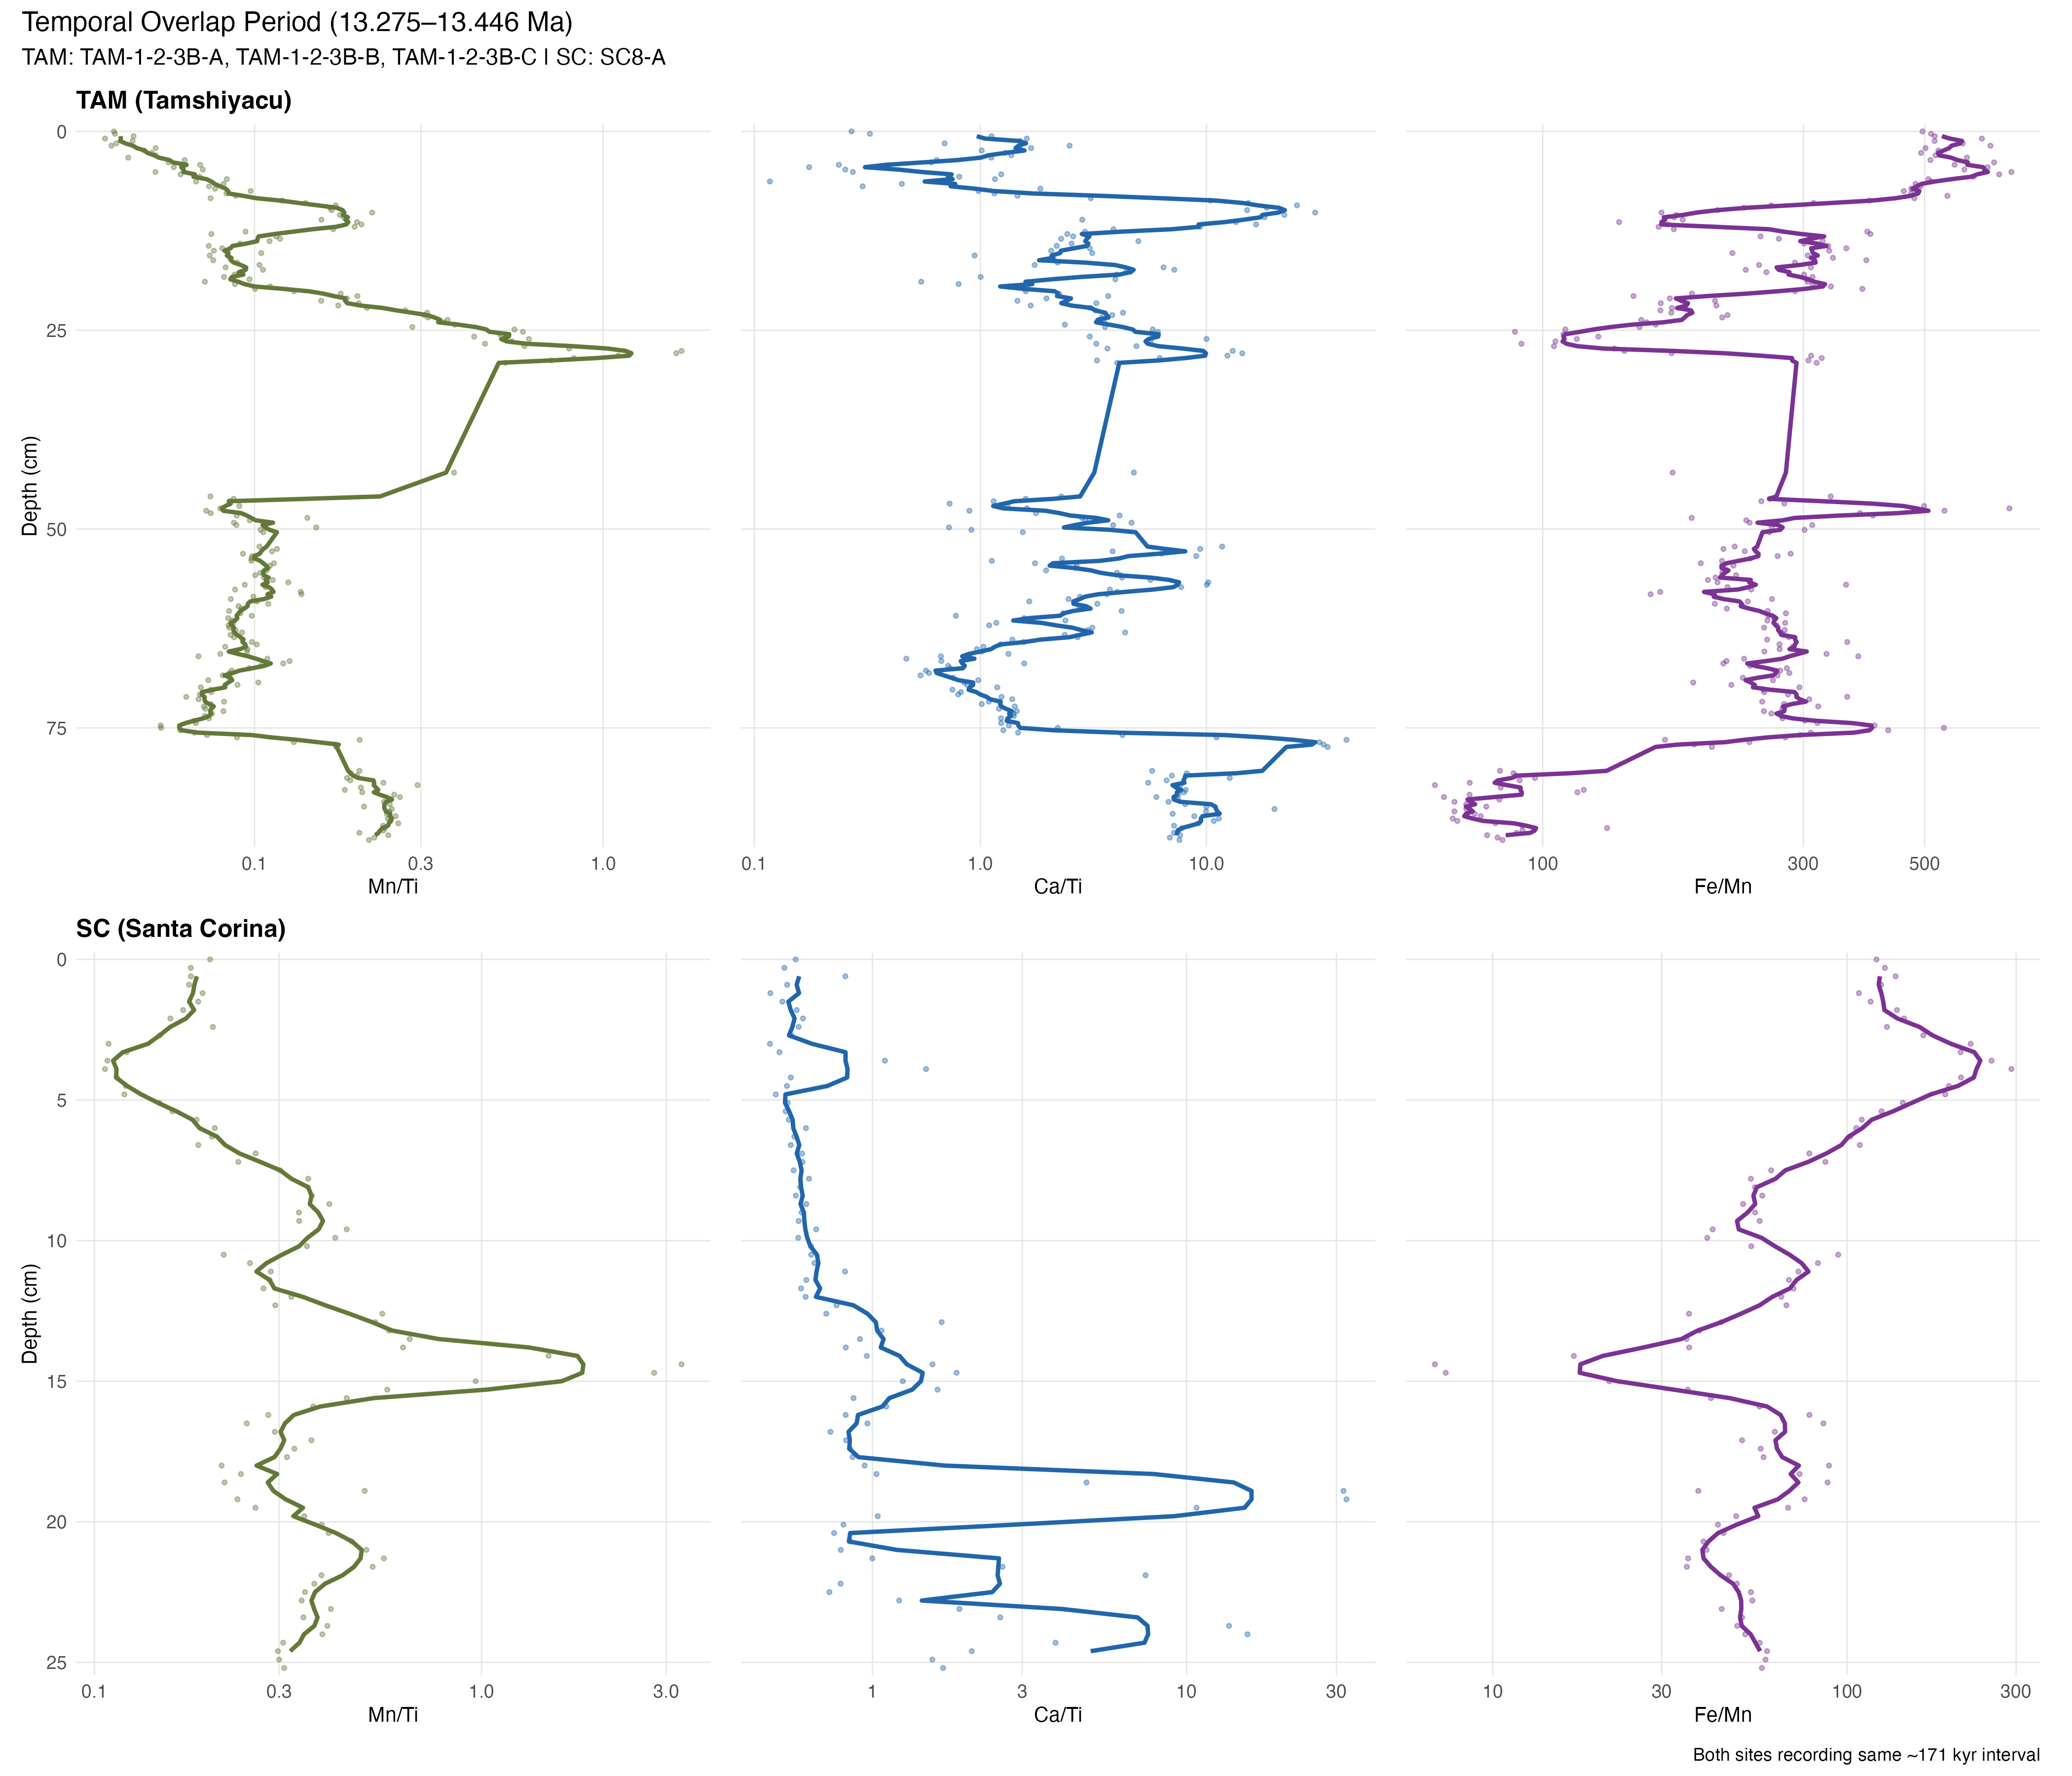
\includegraphics[width=\textwidth]{../output/figures/temporal_overlap/fig5_overlap_comparison.png}
    \caption{Time-equivalent comparison (13.275--13.446 Ma). Top: TAM GROUP1 sections. Bottom: SC8-A. The site contrast persists during the overlap, confirming spatial heterogeneity as the primary driver of proxy differences.}
    \label{fig:overlap-comparison}
\end{figure}

\begin{figure}[H]
    \centering
    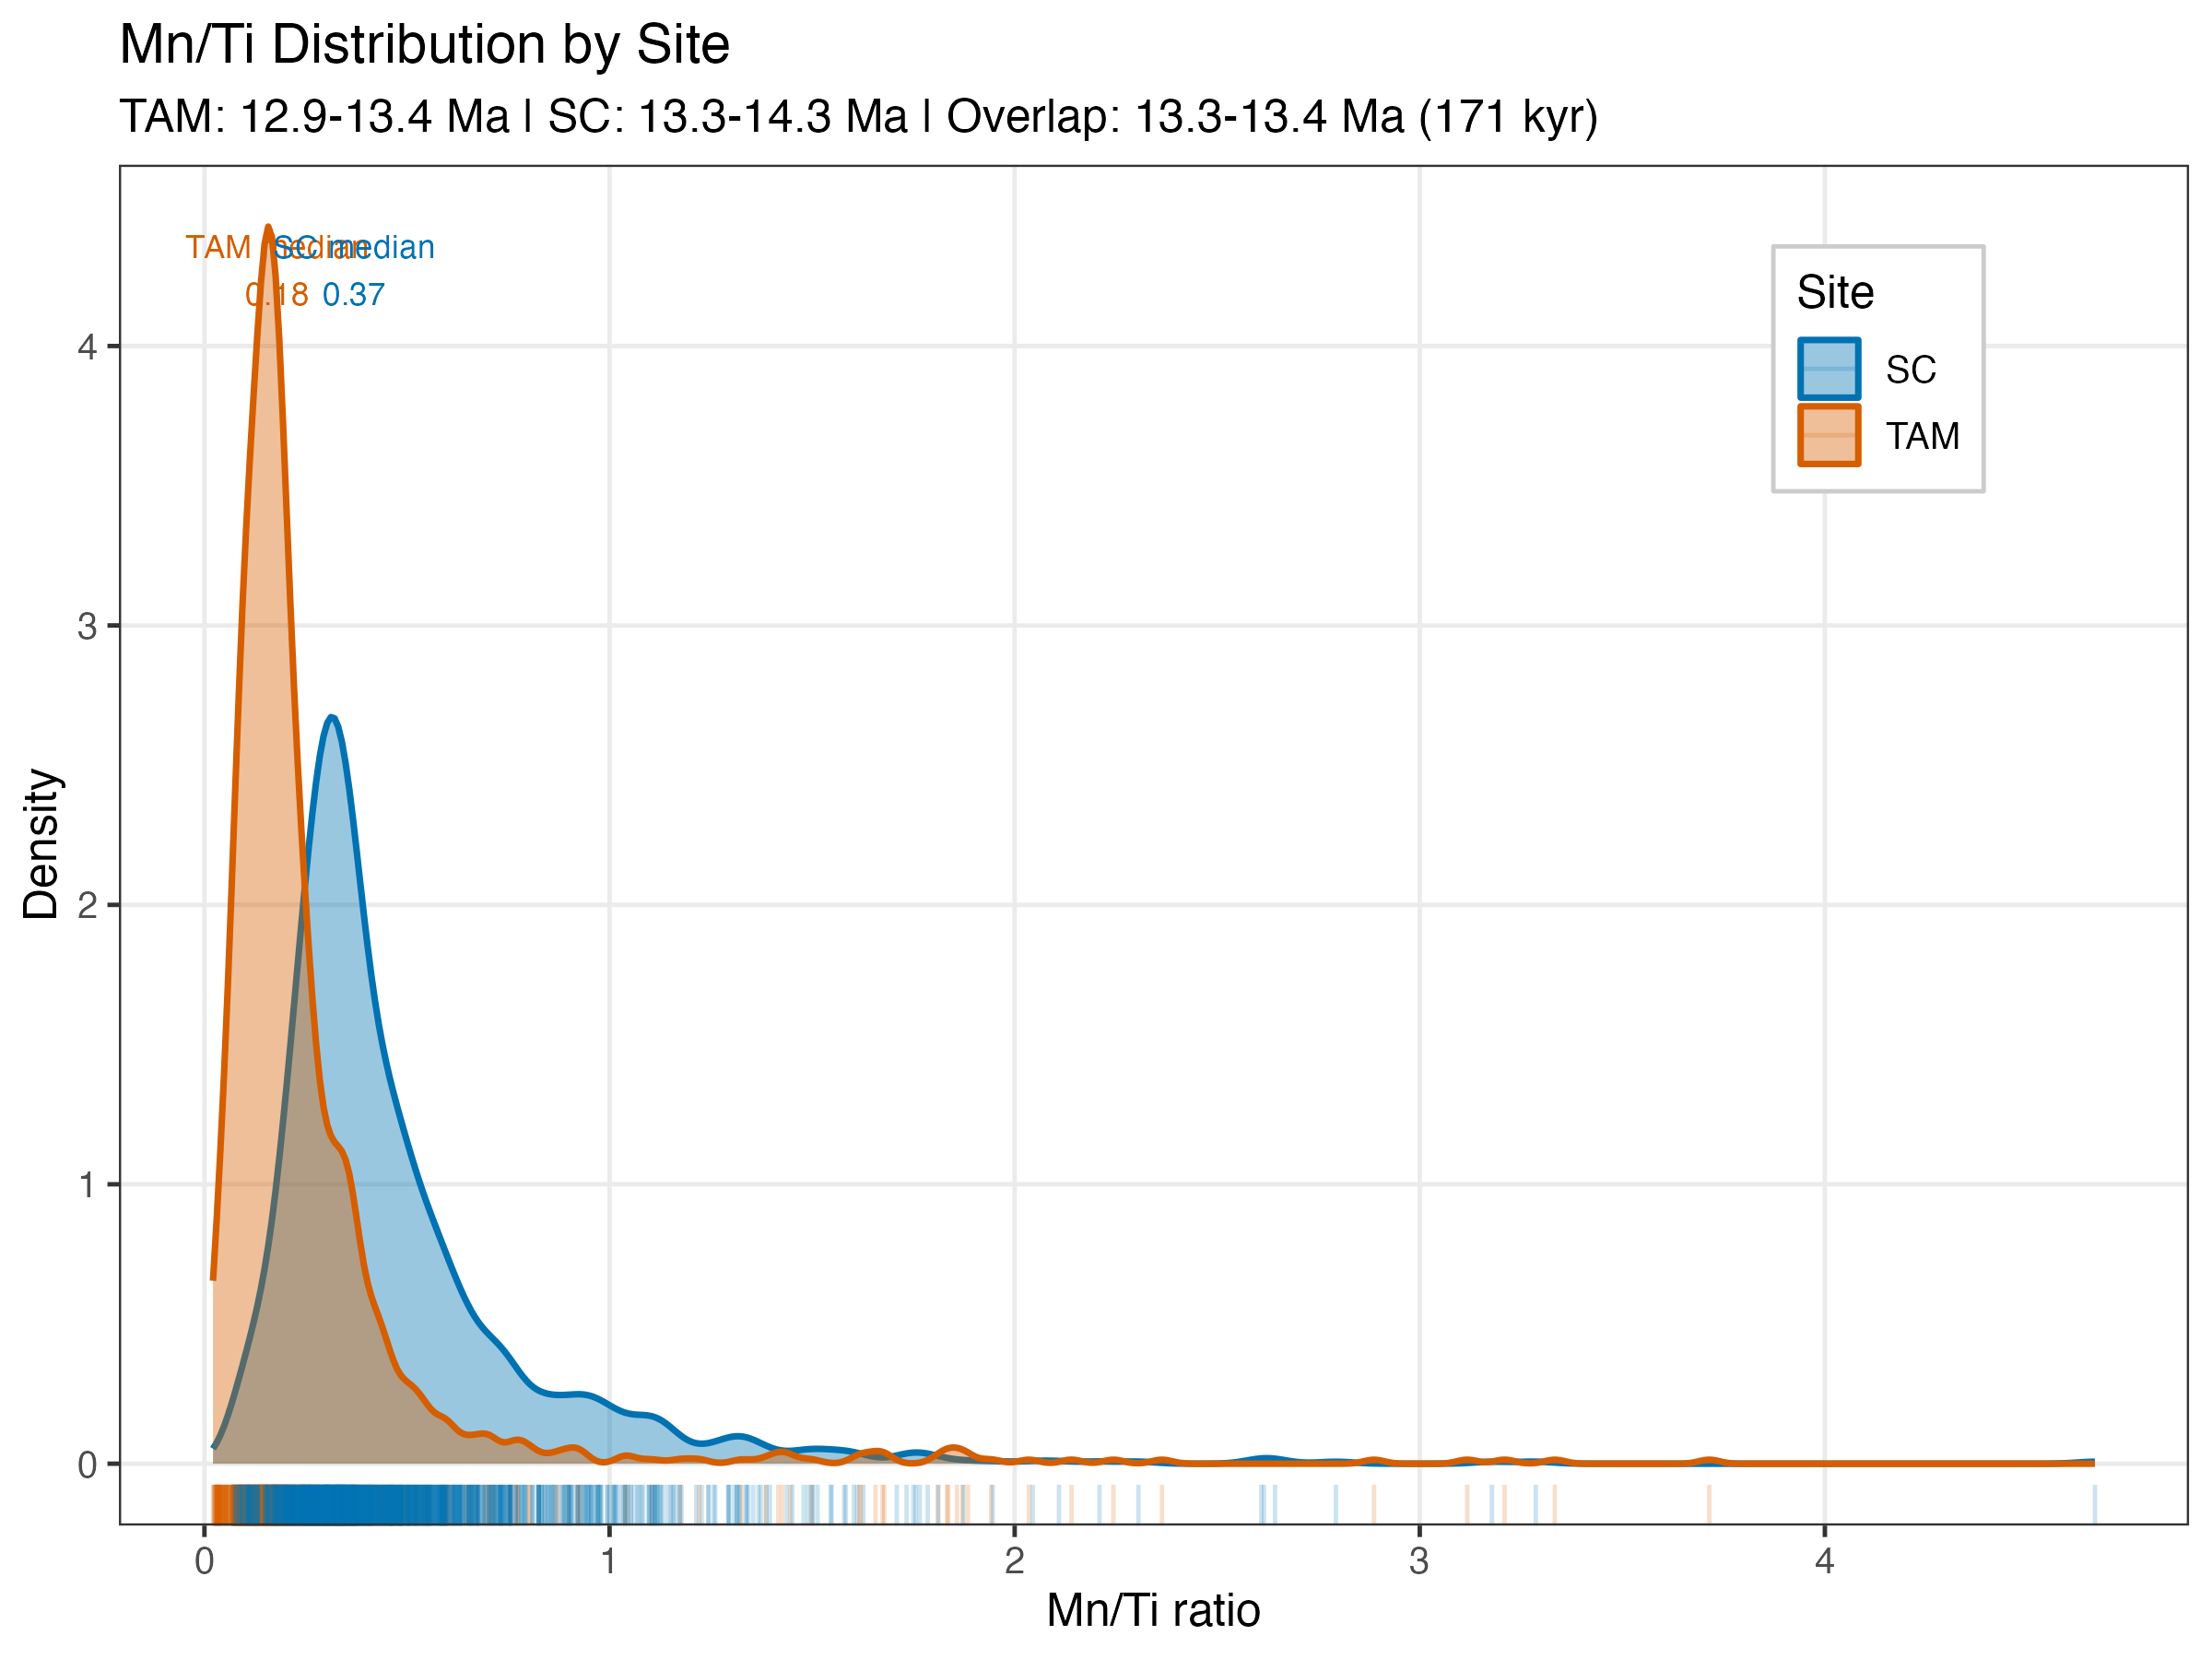
\includegraphics[width=0.85\textwidth]{../output/figures/temporal_overlap/fig1_MnTi_density.png}
    \caption{Mn/Ti distribution comparison. Even during the overlap period, TAM (median 0.18) shows consistently lower Mn/Ti than SC (median 0.37), a 2.1$\times$ difference indicating fundamentally different oxygen regimes.}
    \label{fig:density}
\end{figure}

\begin{tcolorbox}[colback=green!5, colframe=green!50!black, title=Key Finding: Spatial Heterogeneity]
The TAM-SC contrast persists during the temporal overlap, demonstrating that the site difference reflects \textbf{spatial environmental heterogeneity} within the Pebas mega-wetland, not simply temporal evolution.
\begin{itemize}[noitemsep]
    \item TAM = distal, stratified, dysoxic lacustrine setting
    \item SC = proximal, ventilated, fluvio-lacustrine setting
\end{itemize}
\end{tcolorbox}

%==============================================================================
\section{Case Studies: Paleoenvironmental Context}
%==============================================================================

The following case studies highlight specific core intervals that exemplify key paleoenvironmental conditions and their XRF signatures.

\subsection{Case Study 1: Sustained Dysoxia and Exceptional Preservation Potential}

\textbf{Section}: TAM-3A-4-5CDE-A (GROUP2, middle TAM, $\sim$13.1 Ma)

\textbf{Paleoenvironmental context}: This interval represents the classic ``taphonomic sweet spot'' of the Pebas system---sustained low-oxygen conditions that inhibit scavenging and bioturbation while promoting organic matter preservation.

\begin{figure}[H]
    \centering
    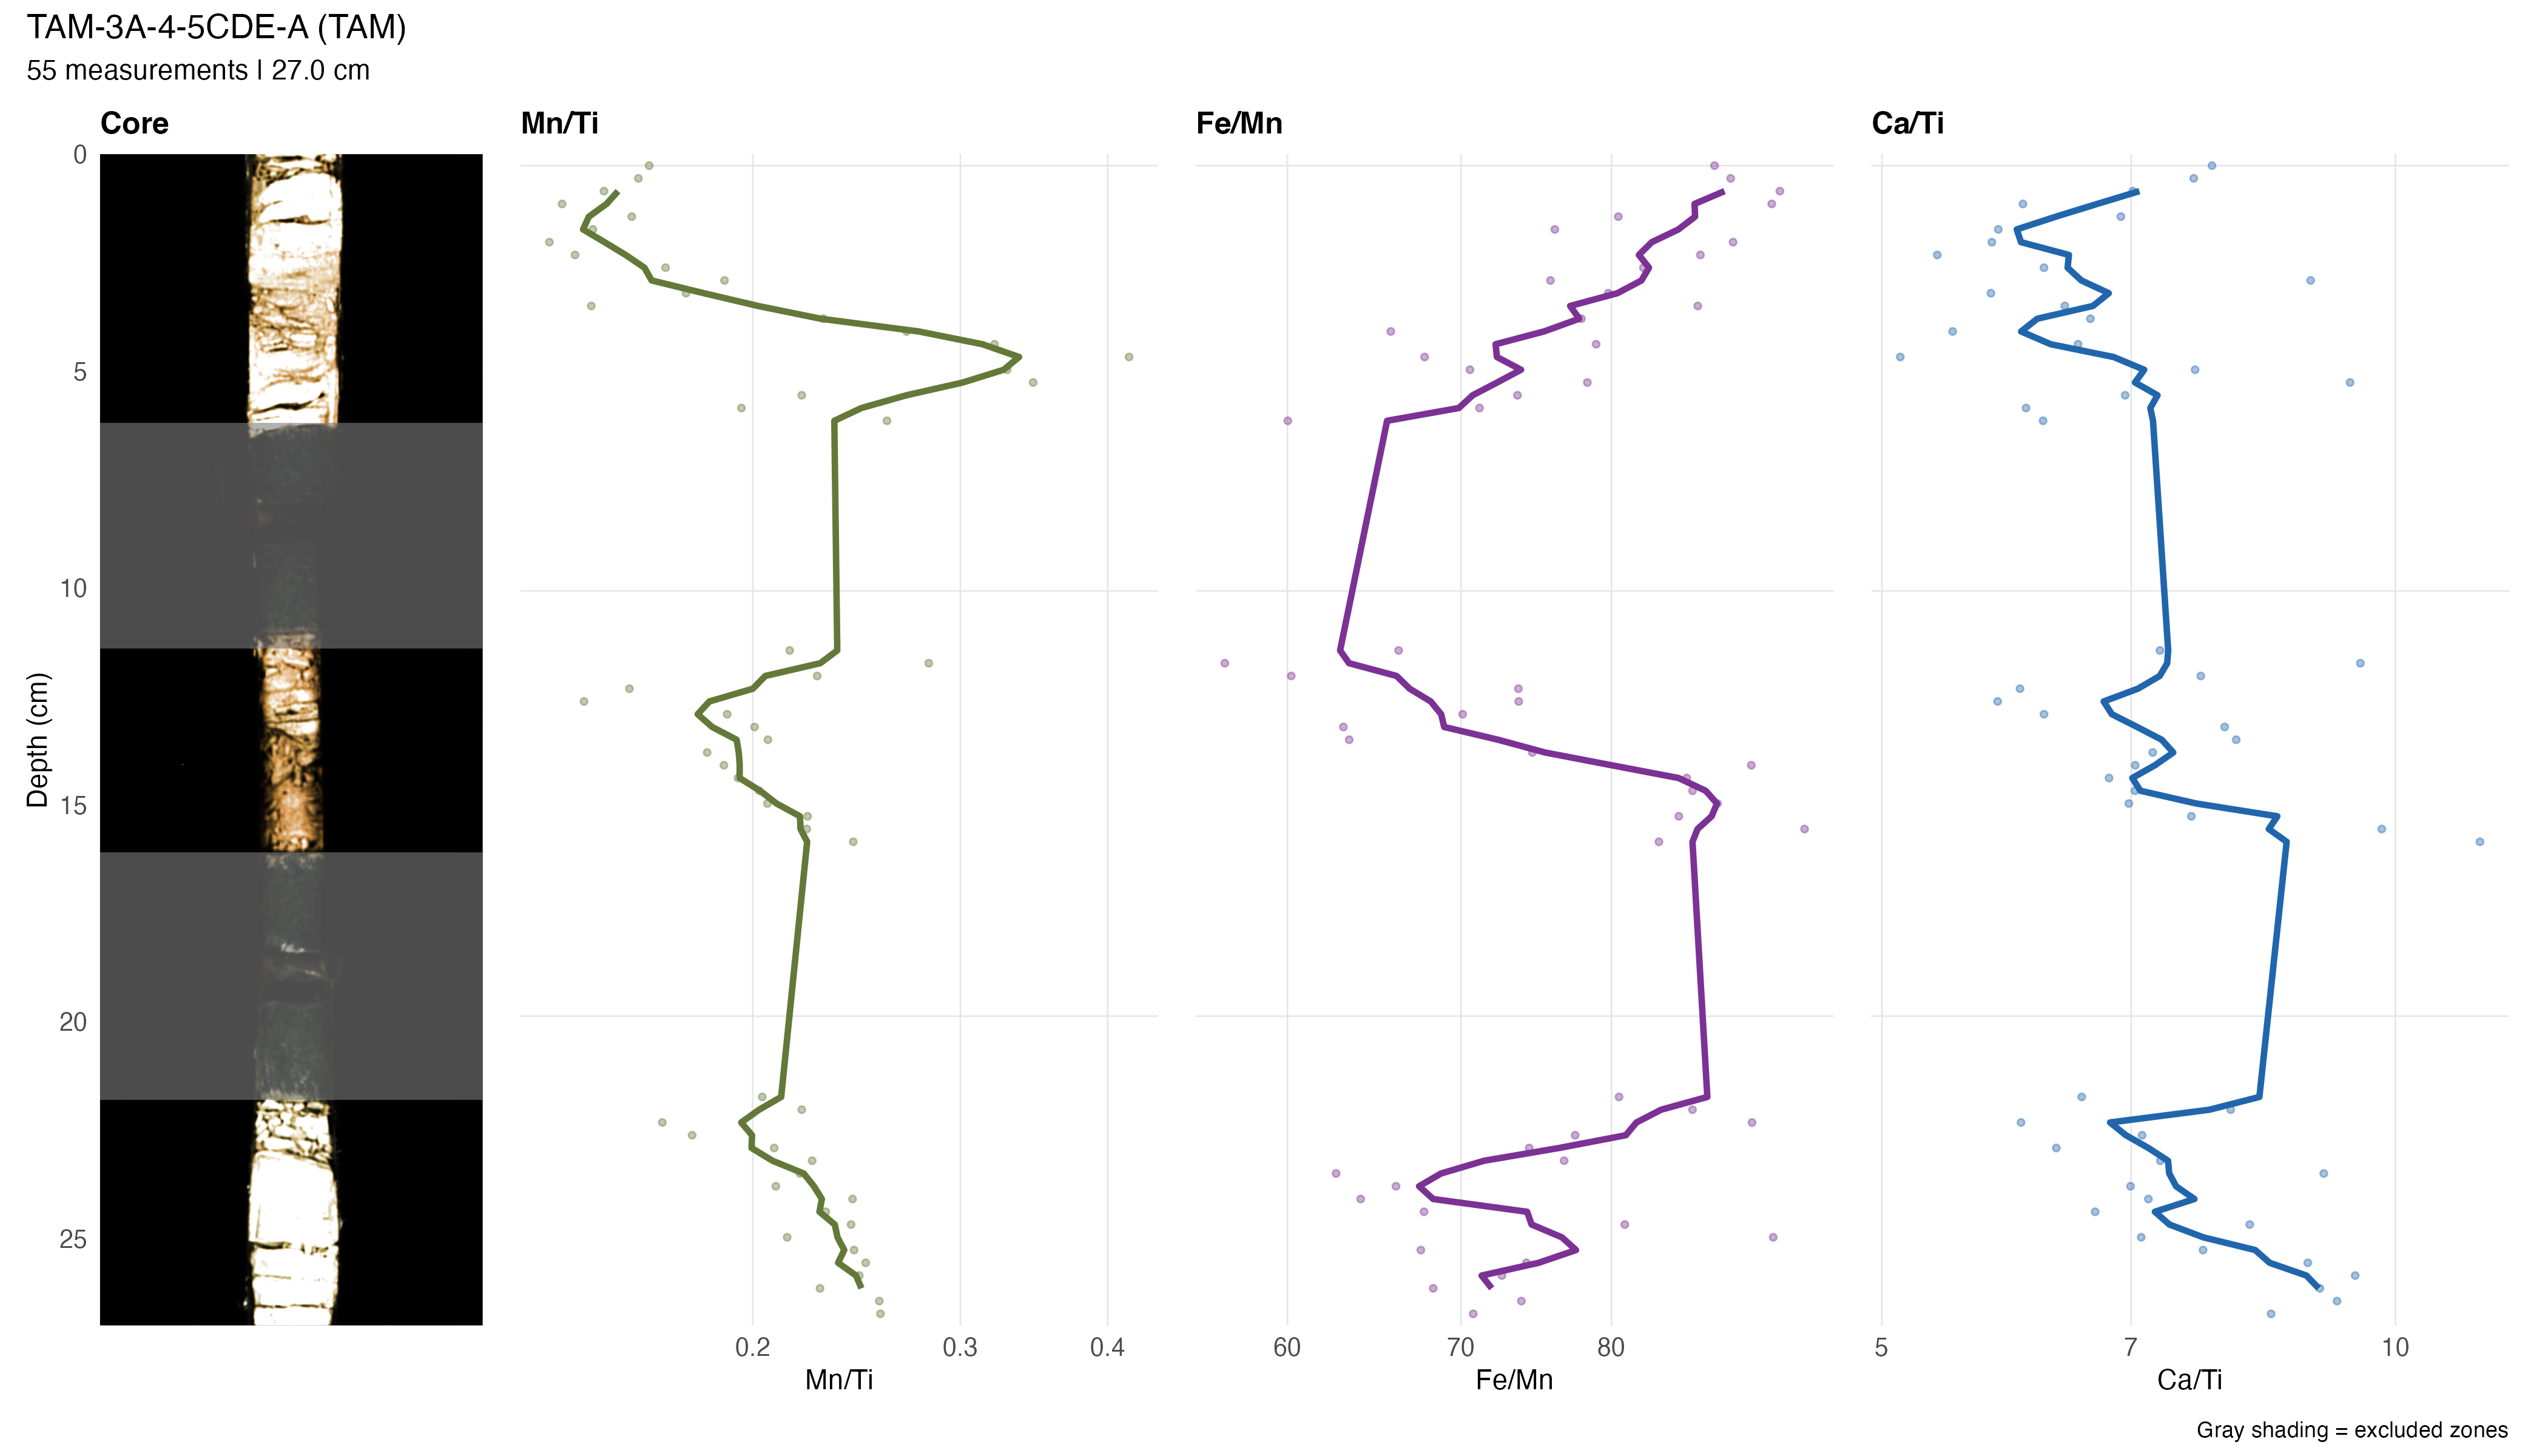
\includegraphics[width=\textwidth]{../output/figures/temporal_overlap/case1_anoxic_TAM-3A-4-5CDE-A.png}
    \caption{TAM-3A-4-5CDE-A: Sustained dysoxic interval. Dark, organic-rich sediment correlates with low Mn/Ti. Periodic lighter bands represent brief oxygenation events. This interval would favor articulated fossil preservation.}
    \label{fig:case-dysoxia}
\end{figure}

\textbf{Preservation implications}:
\begin{itemize}
    \item Mn/Ti $<$ 0.15 indicates bottom-water O$_2$ $<$ 0.2 ml/L
    \item Fe/Mn $>$ 100 confirms strongly reducing conditions
    \item \textit{Pachydon obliquus} habitat---the dysoxia-tolerant bivalve indicator
    \item Optimal for: articulated vertebrates, complete mollusc assemblages, soft tissue traces
\end{itemize}

\subsection{Case Study 2: Carbonate-Rich Shell Beds}

\textbf{Section}: SC-3AB-4ABCD-A (GROUP5, middle SC, $\sim$13.6 Ma)

\textbf{Paleoenvironmental context}: This interval shows pronounced Ca/Ti peaks indicating concentrated mollusc shell accumulation. These shell beds provide insight into productivity events and alkaline water conditions.

\begin{figure}[H]
    \centering
    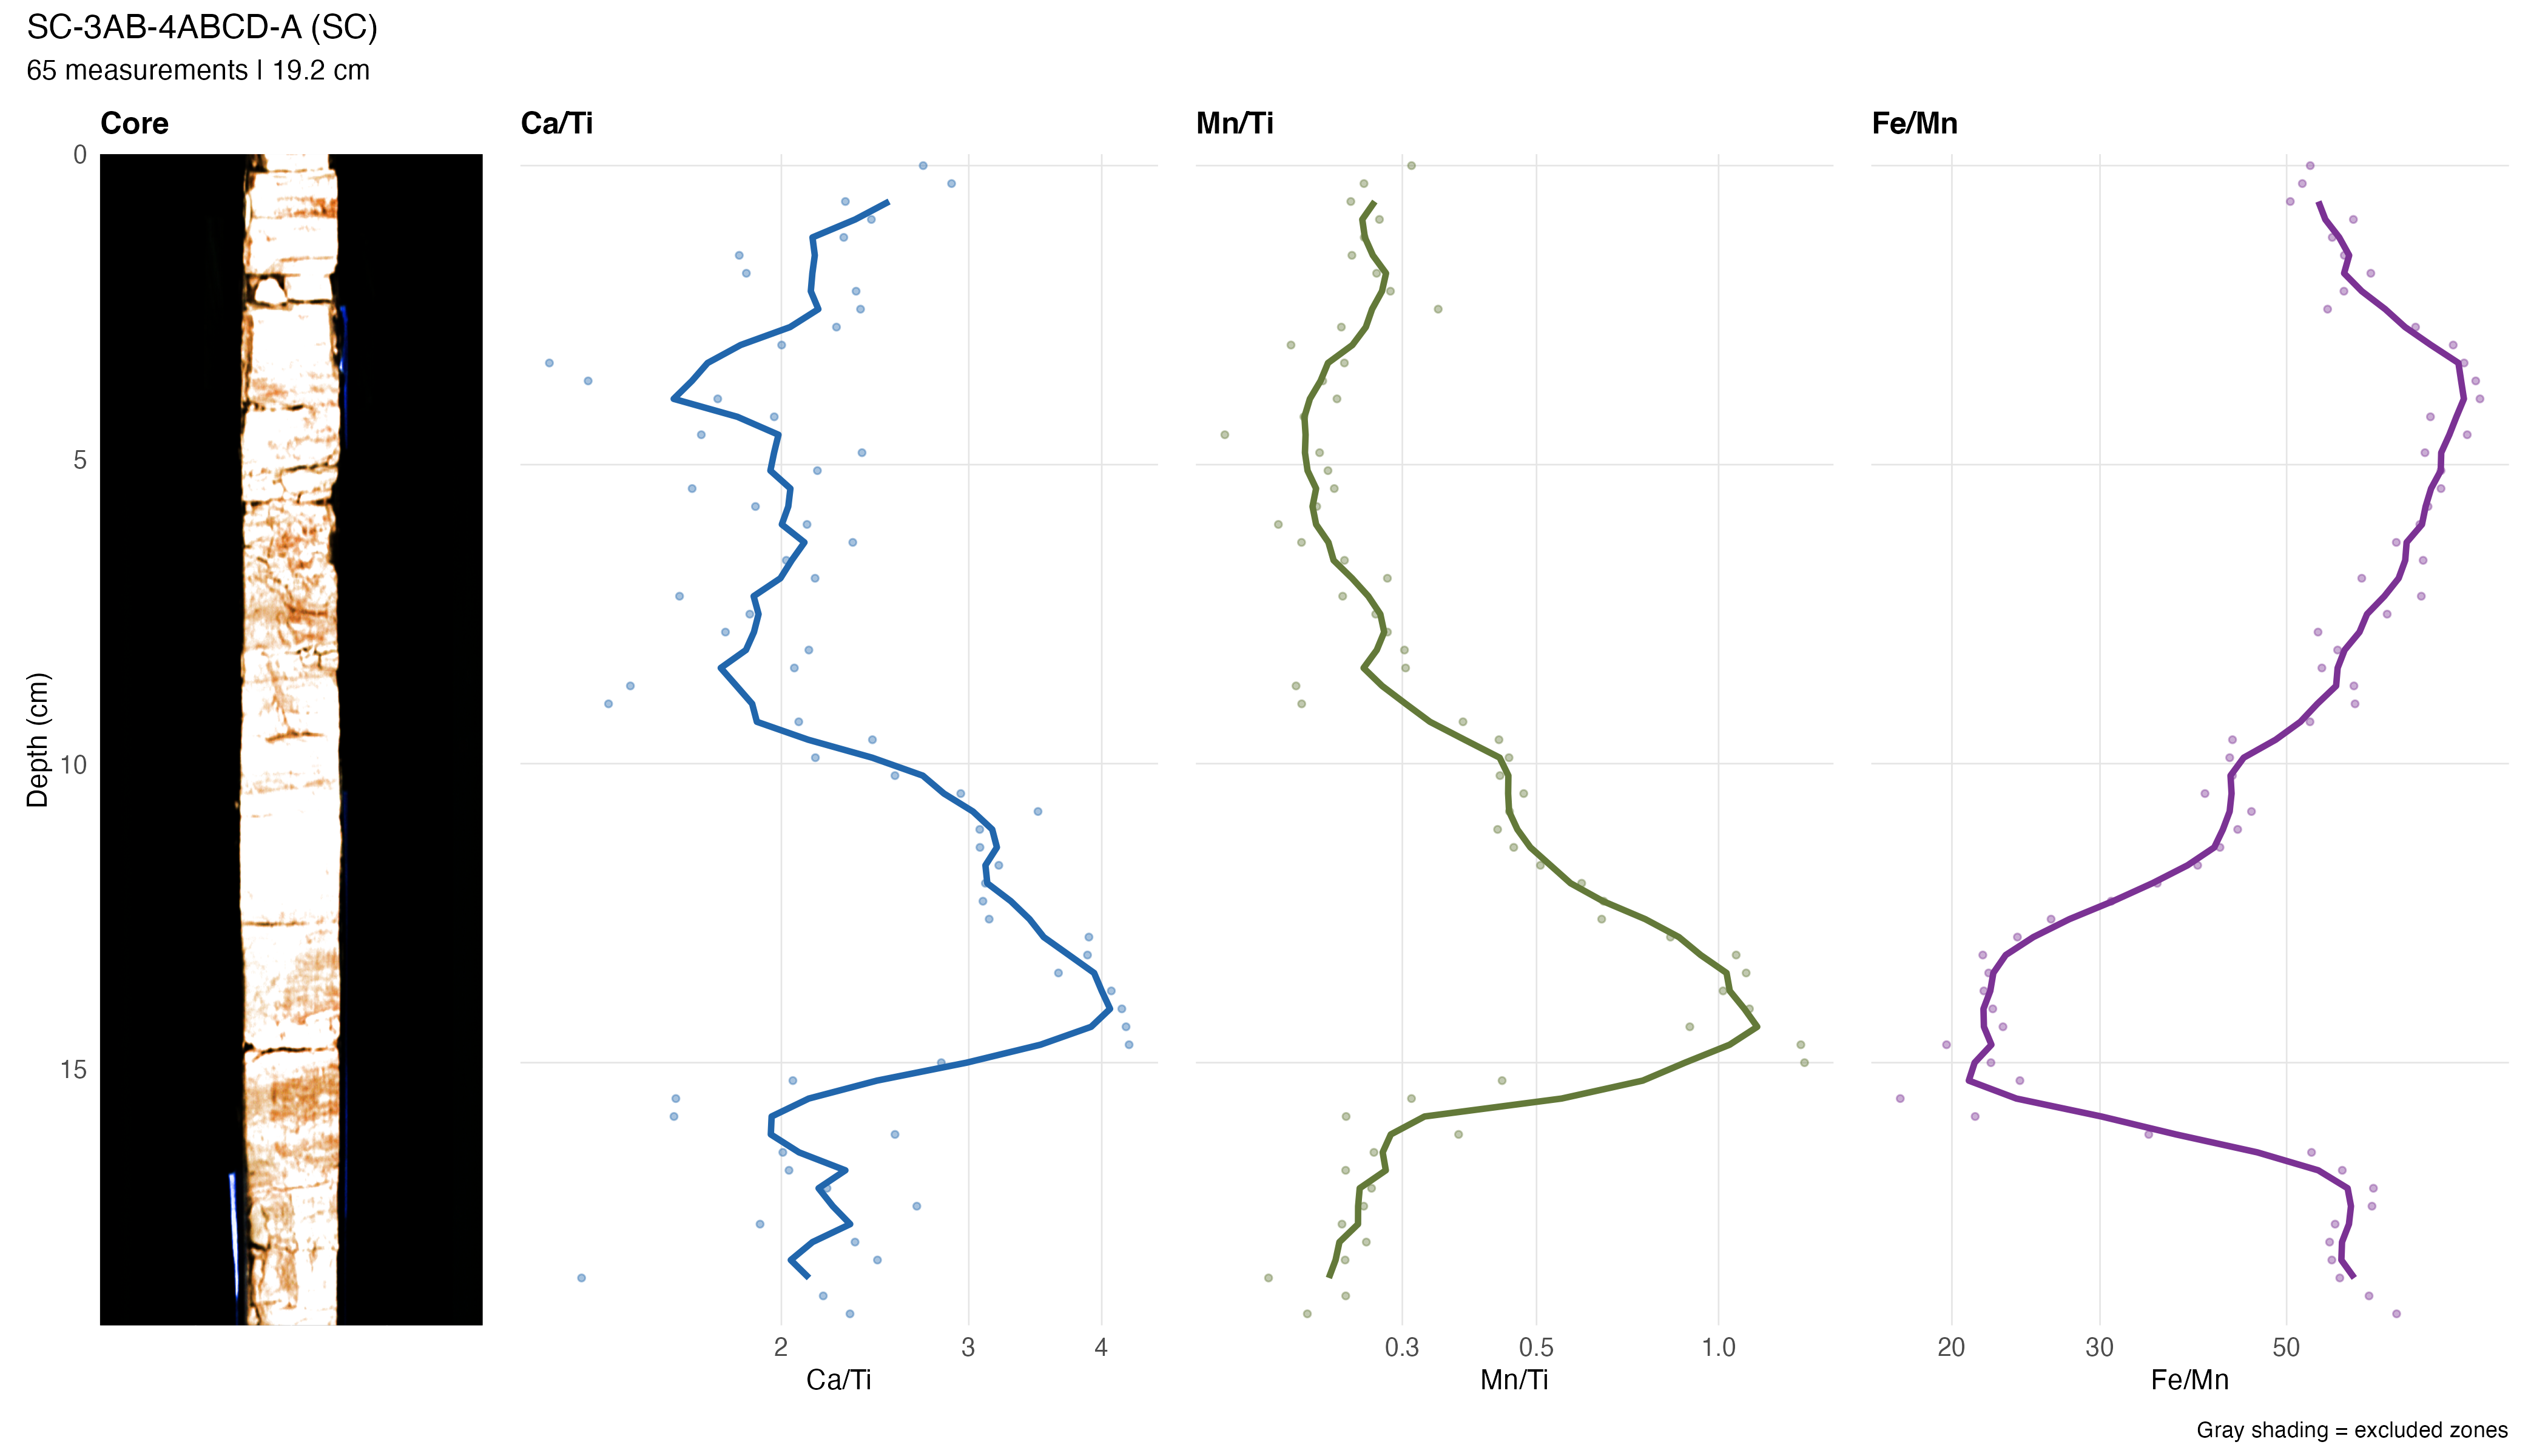
\includegraphics[width=\textwidth]{../output/figures/temporal_overlap/case2_carbonate_SC-3AB-4ABCD-A.png}
    \caption{SC-3AB-4ABCD-A: Shell-rich interval. Ca/Ti peaks correspond to visible lighter, shell-rich horizons in the core image. Note that some Ca/Ti peaks occur with high Mn/Ti (oxic conditions favoring in-situ mollusc communities) while others occur with low Mn/Ti (transported shells into dysoxic zones).}
    \label{fig:case-carbonate}
\end{figure}

\textbf{Paleoenvironmental interpretation}:
\begin{itemize}
    \item High Ca/Ti + high Mn/Ti = in-situ mollusc community under oxic conditions
    \item High Ca/Ti + low Mn/Ti = shell transport into dysoxic setting (storm events, mass mortality)
    \item Ca/Ti variability indicates episodic productivity or transport events
    \item Shell preservation suggests alkaline waters (high pH preventing dissolution)
\end{itemize}

\subsection{Case Study 3: Environmental Transition}

\textbf{Section}: TAM-5AB-6-7-A (GROUP3, youngest TAM interval, $\sim$12.95 Ma)

\textbf{Paleoenvironmental context}: This section captures subtle shifts in proxy relationships that may record the late-stage evolution of Pebas lacustrine conditions before eventual drainage.

\begin{figure}[H]
    \centering
    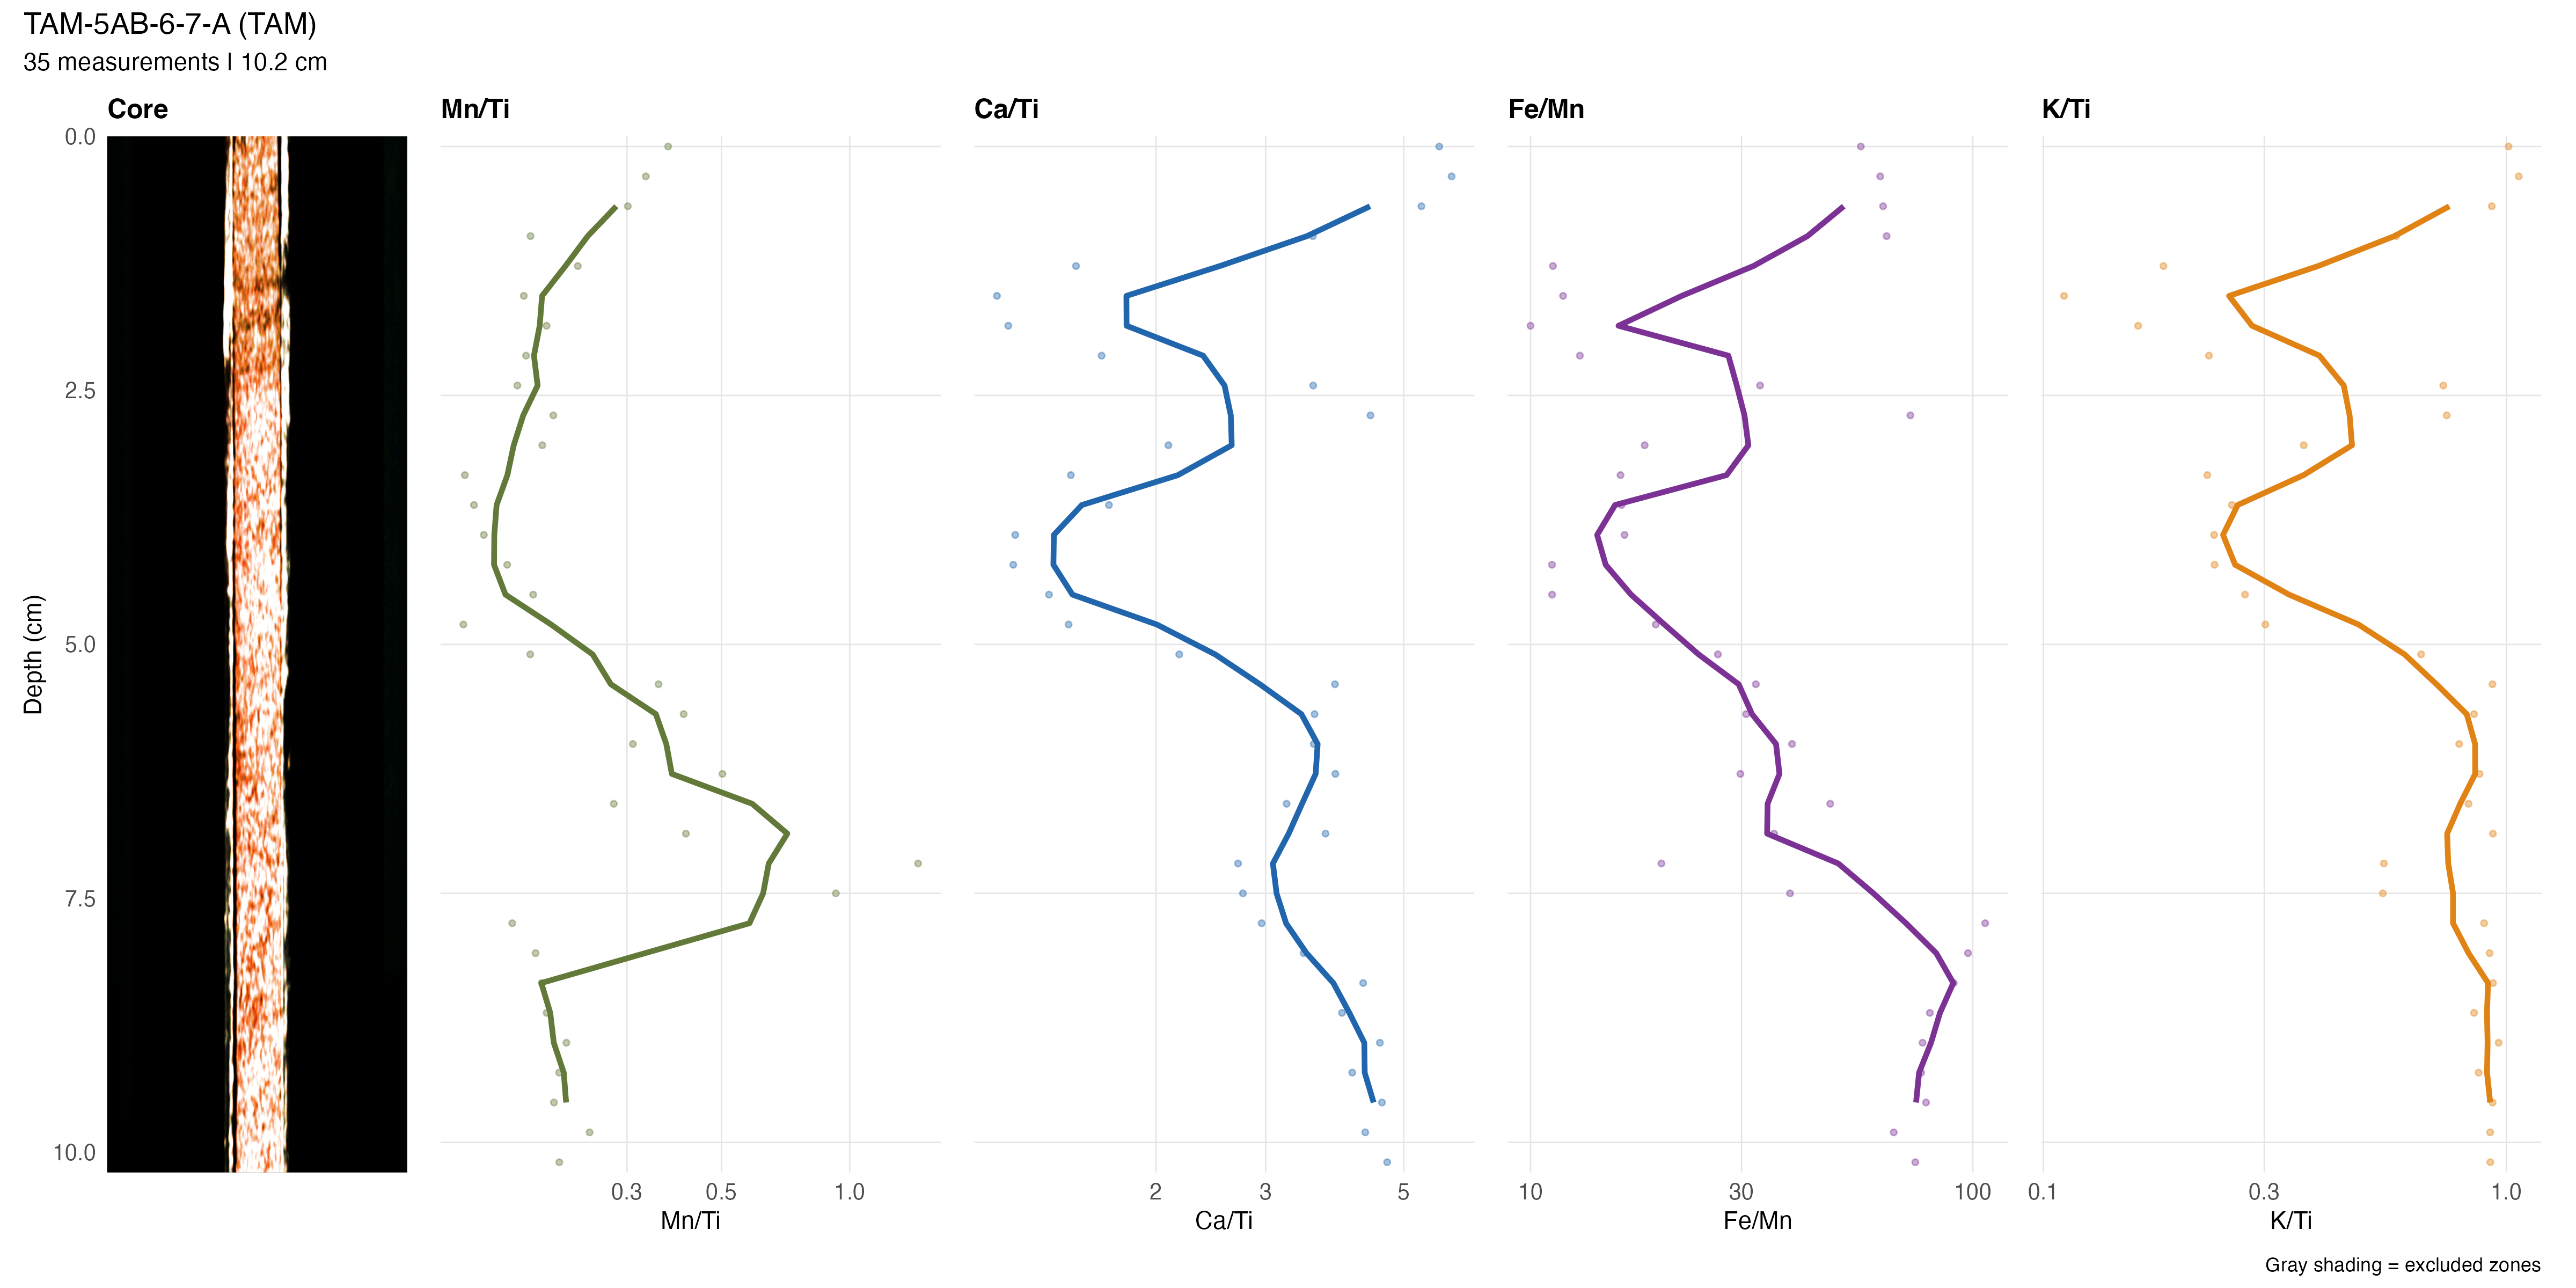
\includegraphics[width=\textwidth]{../output/figures/temporal_overlap/case3_transition_TAM-5AB-6-7-A.png}
    \caption{TAM-5AB-6-7-A: Environmental transition interval. Note how proxy relationships change through the section, potentially recording shifts in stratification, input sources, or lake-level changes.}
    \label{fig:case-transition}
\end{figure}

\textbf{Dynamic interpretation}:
\begin{itemize}
    \item Variable Mn/Ti suggests fluctuating oxygen conditions
    \item K/Ti variations may indicate changing weathering intensity or sediment provenance
    \item This youngest TAM interval may capture environmental instability preceding later Pebas drainage
\end{itemize}

\subsection{Case Study 4: High-Frequency Redox Oscillations}

\textbf{Section}: SC-5-6-7ABC-A (GROUP6, younger SC, $\sim$13.4 Ma)

\textbf{Paleoenvironmental context}: This section shows remarkably high-frequency oscillations in redox proxies, potentially reflecting seasonal or sub-decadal environmental variability.

\begin{figure}[H]
    \centering
    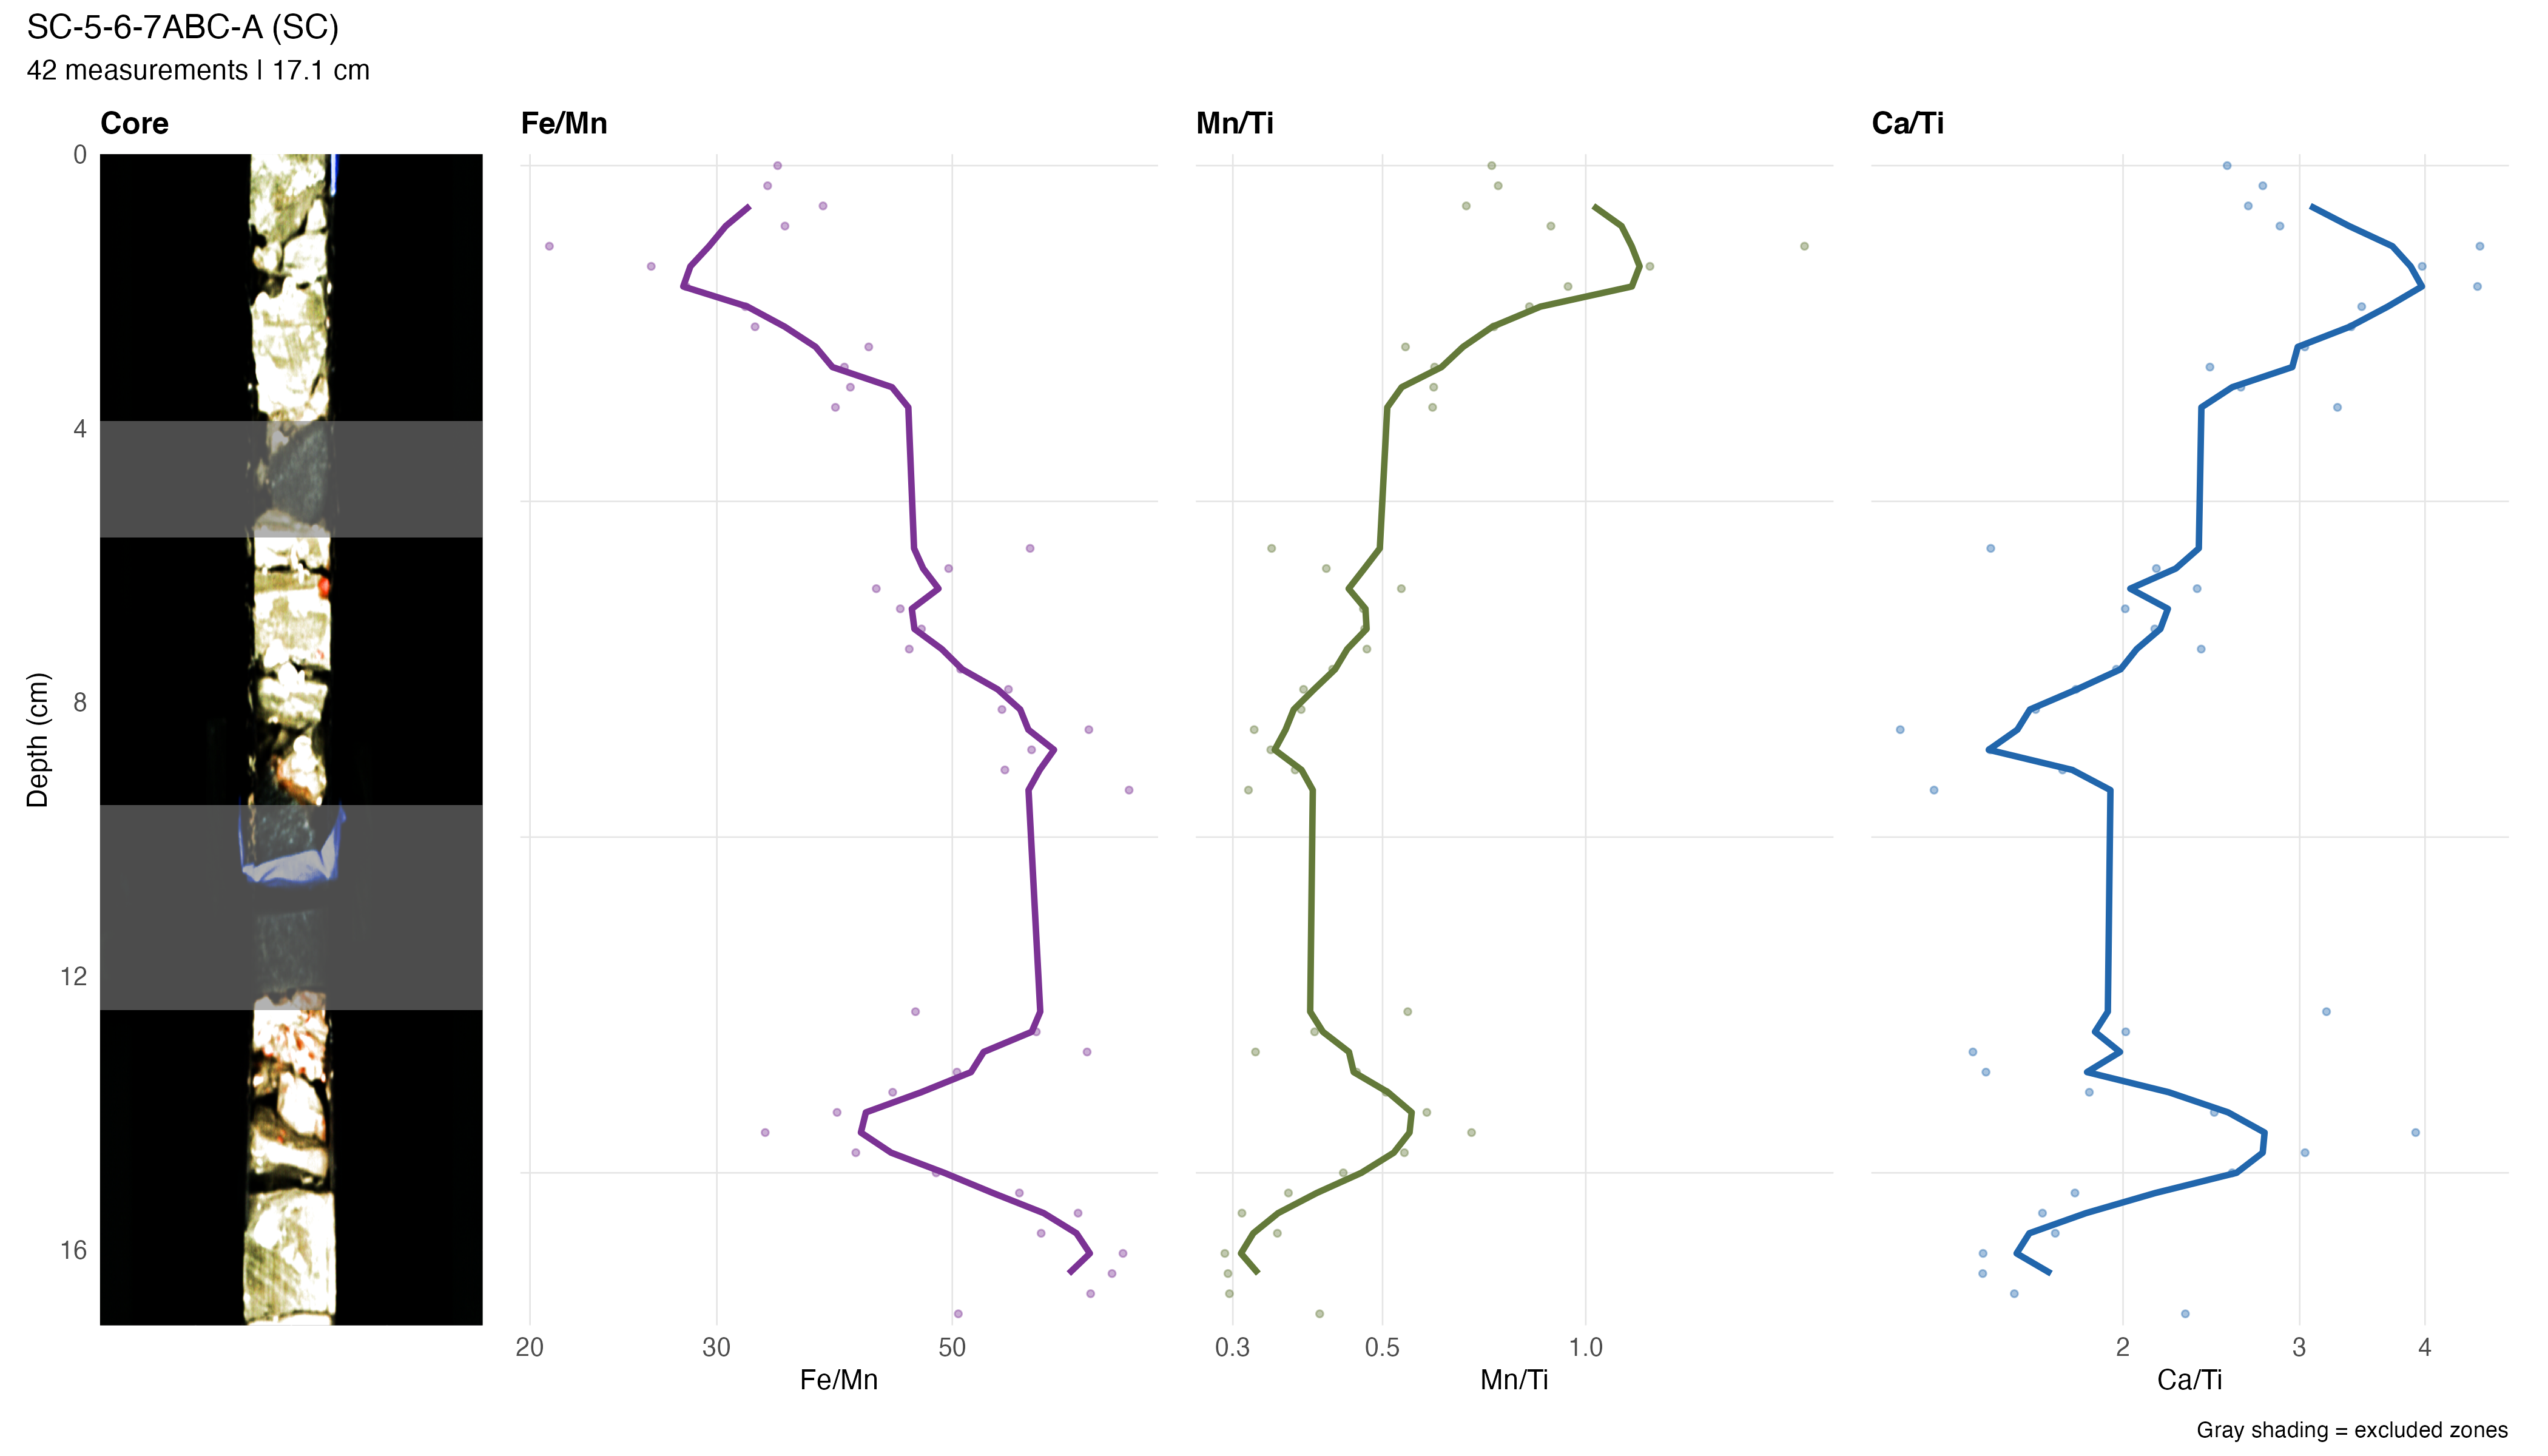
\includegraphics[width=\textwidth]{../output/figures/temporal_overlap/case4_redox_SC-5-6-7ABC-A.png}
    \caption{SC-5-6-7ABC-A: High-frequency redox variability. The anti-correlation between Fe/Mn and Mn/Ti confirms these are genuine redox signals. Oscillation frequency may reflect seasonal mixing cycles or flood-induced ventilation events.}
    \label{fig:case-redox}
\end{figure}

\textbf{Environmental dynamics}:
\begin{itemize}
    \item High Fe/Mn = reducing conditions (Fe mobile, Mn depleted)
    \item Low Fe/Mn = oxic conditions (Mn precipitates as MnO$_2$)
    \item Oscillation wavelength: $\sim$10--20 mm $\approx$ 50--100 years (at SC sed rate)
    \item Possible drivers: seasonal stratification/mixing, flood pulses, lake-level changes
\end{itemize}

\subsection{Case Study 5: Oldest SC---Deep-Time Baseline}

\textbf{Section}: SC-1ABC-2-3C-A-RUN1 (GROUP4, oldest SC, $\sim$14.3 Ma)

\textbf{Paleoenvironmental context}: This oldest SC section provides the deep-time baseline, recording Pebas conditions nearly 1.4 million years before the youngest TAM sediments.

\begin{figure}[H]
    \centering
    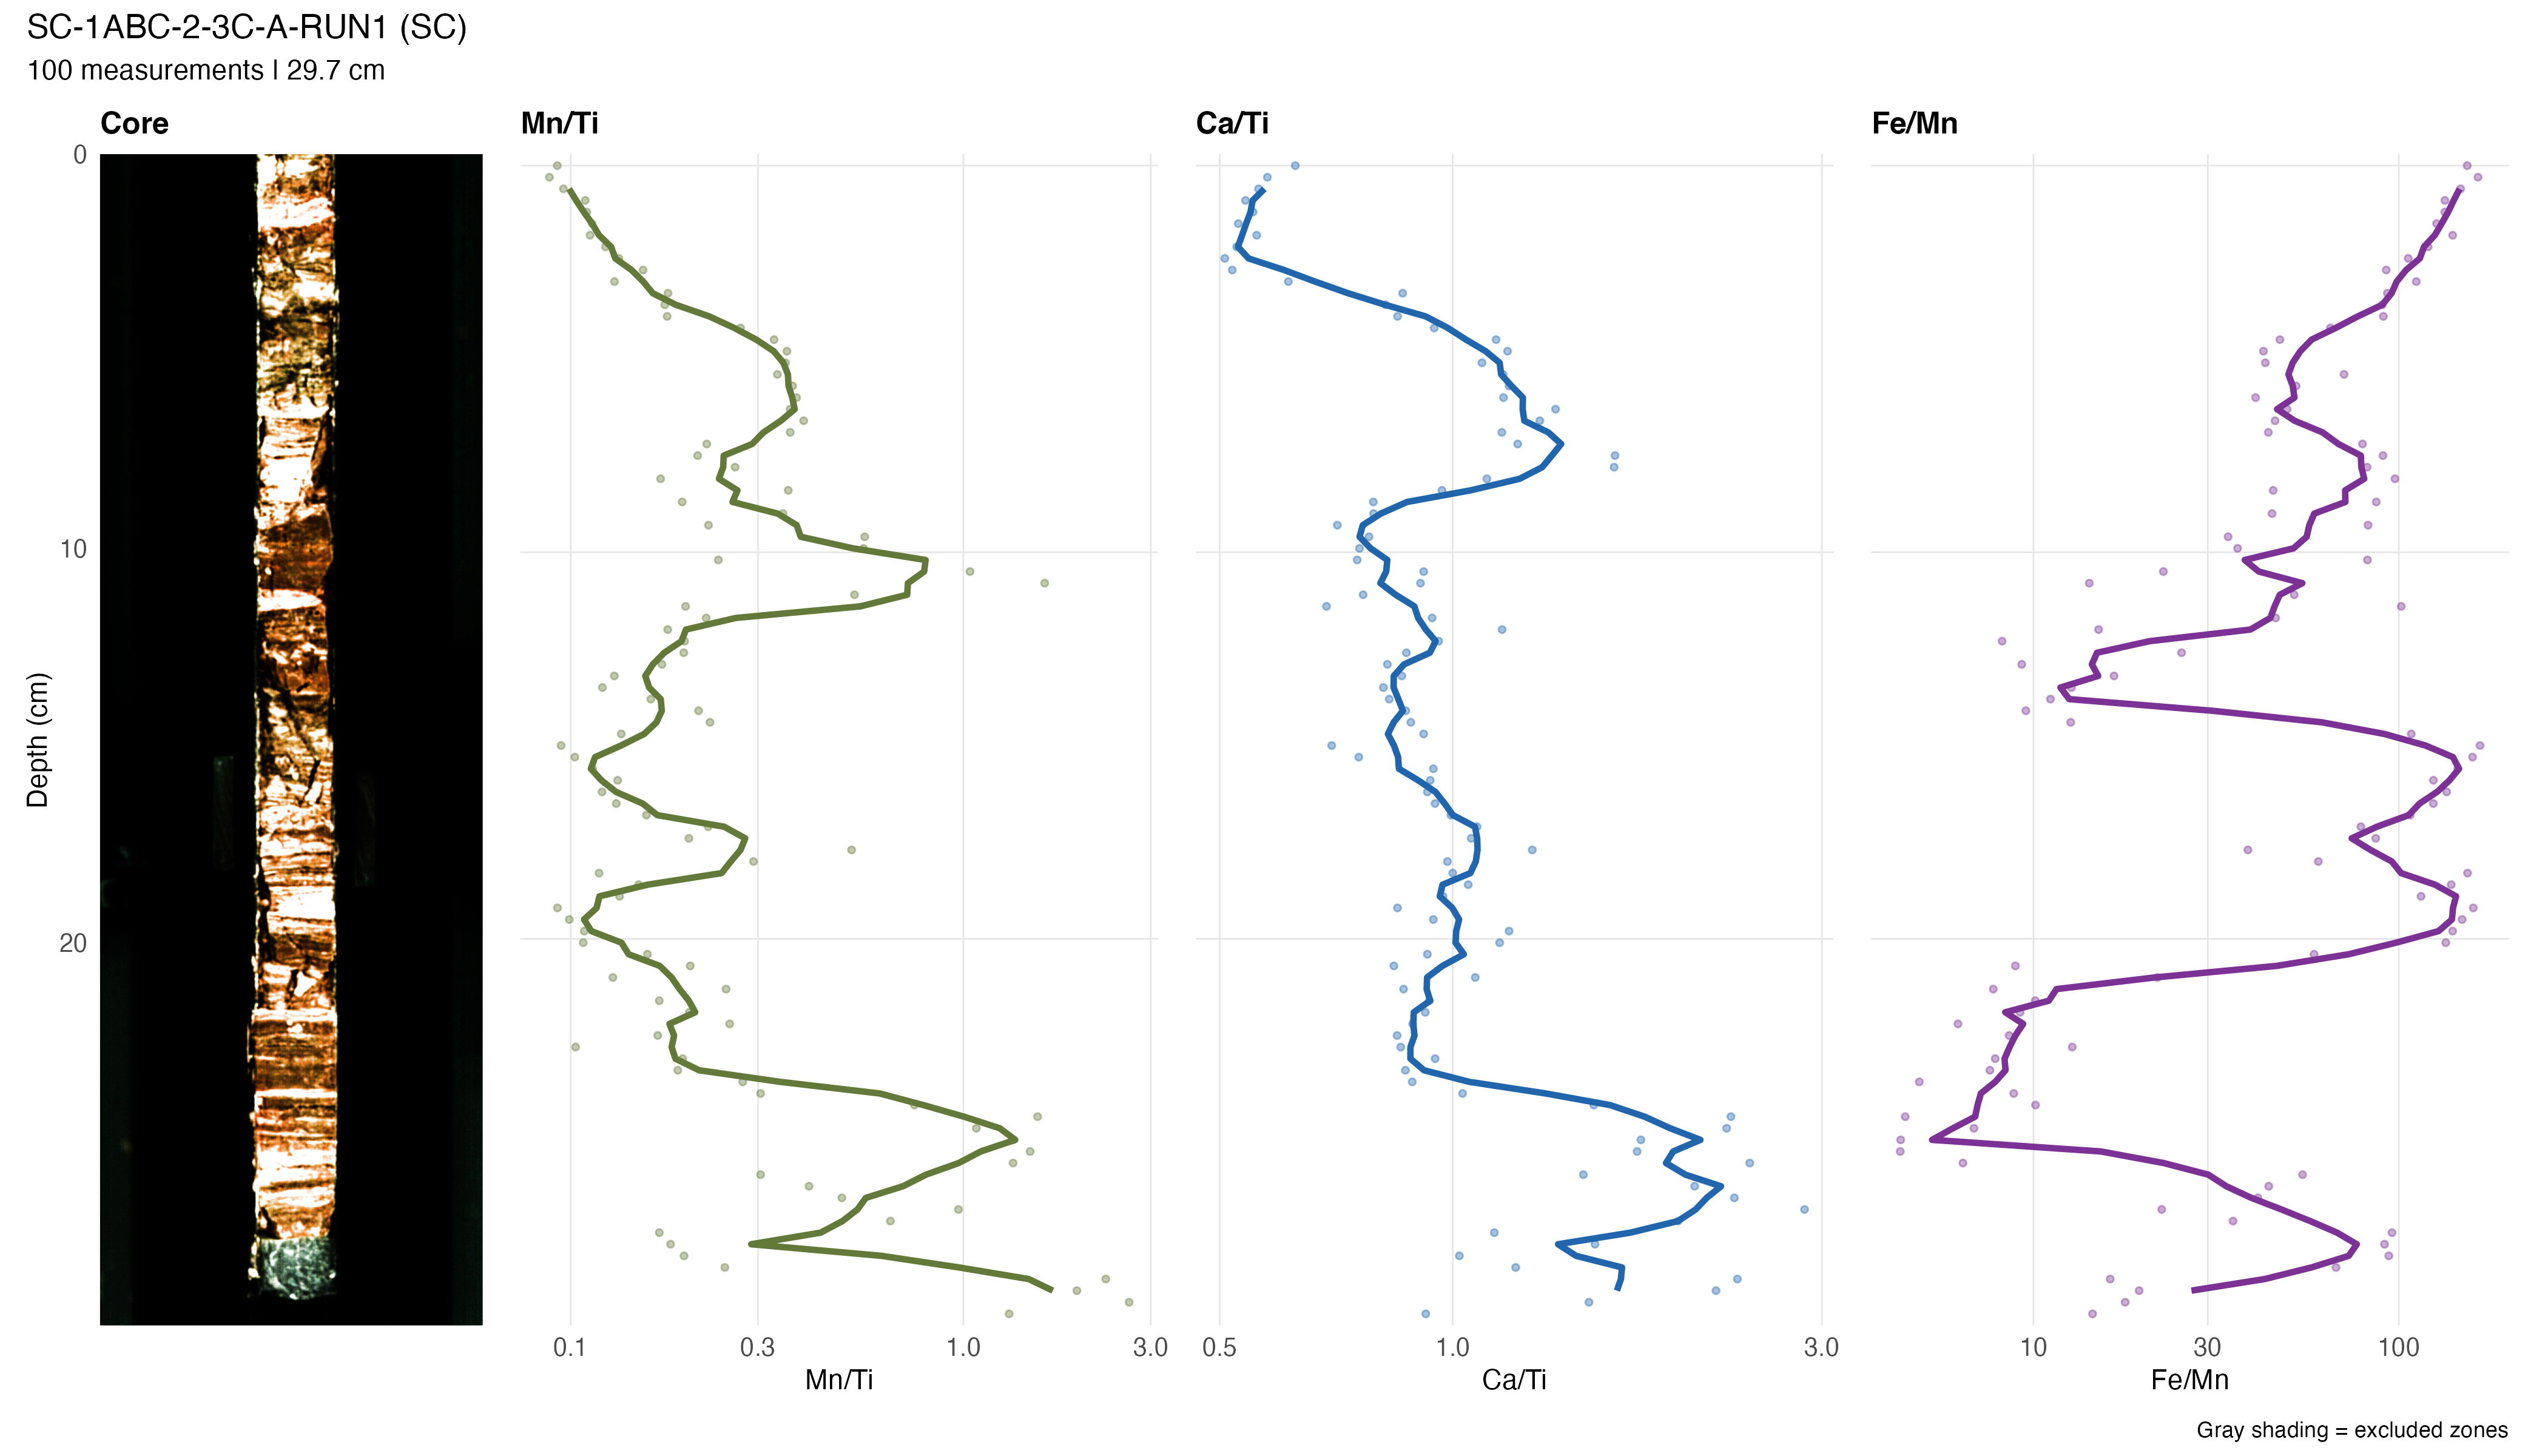
\includegraphics[width=\textwidth]{../output/figures/temporal_overlap/bottom_SC-1ABC-2-3C-A-RUN1.png}
    \caption{SC-1ABC-2-3C-A-RUN1: Oldest SC section ($\sim$14.3 Ma). This deep-time record shows the SC site already exhibited the ventilated, variable character seen throughout its younger sections, suggesting long-term stability of site-specific environmental conditions.}
    \label{fig:sc-oldest}
\end{figure}

%==============================================================================
\section{Synthesis: Paleoenvironmental Model}
%==============================================================================

\subsection{Environmental Modes}

\begin{figure}[H]
    \centering
    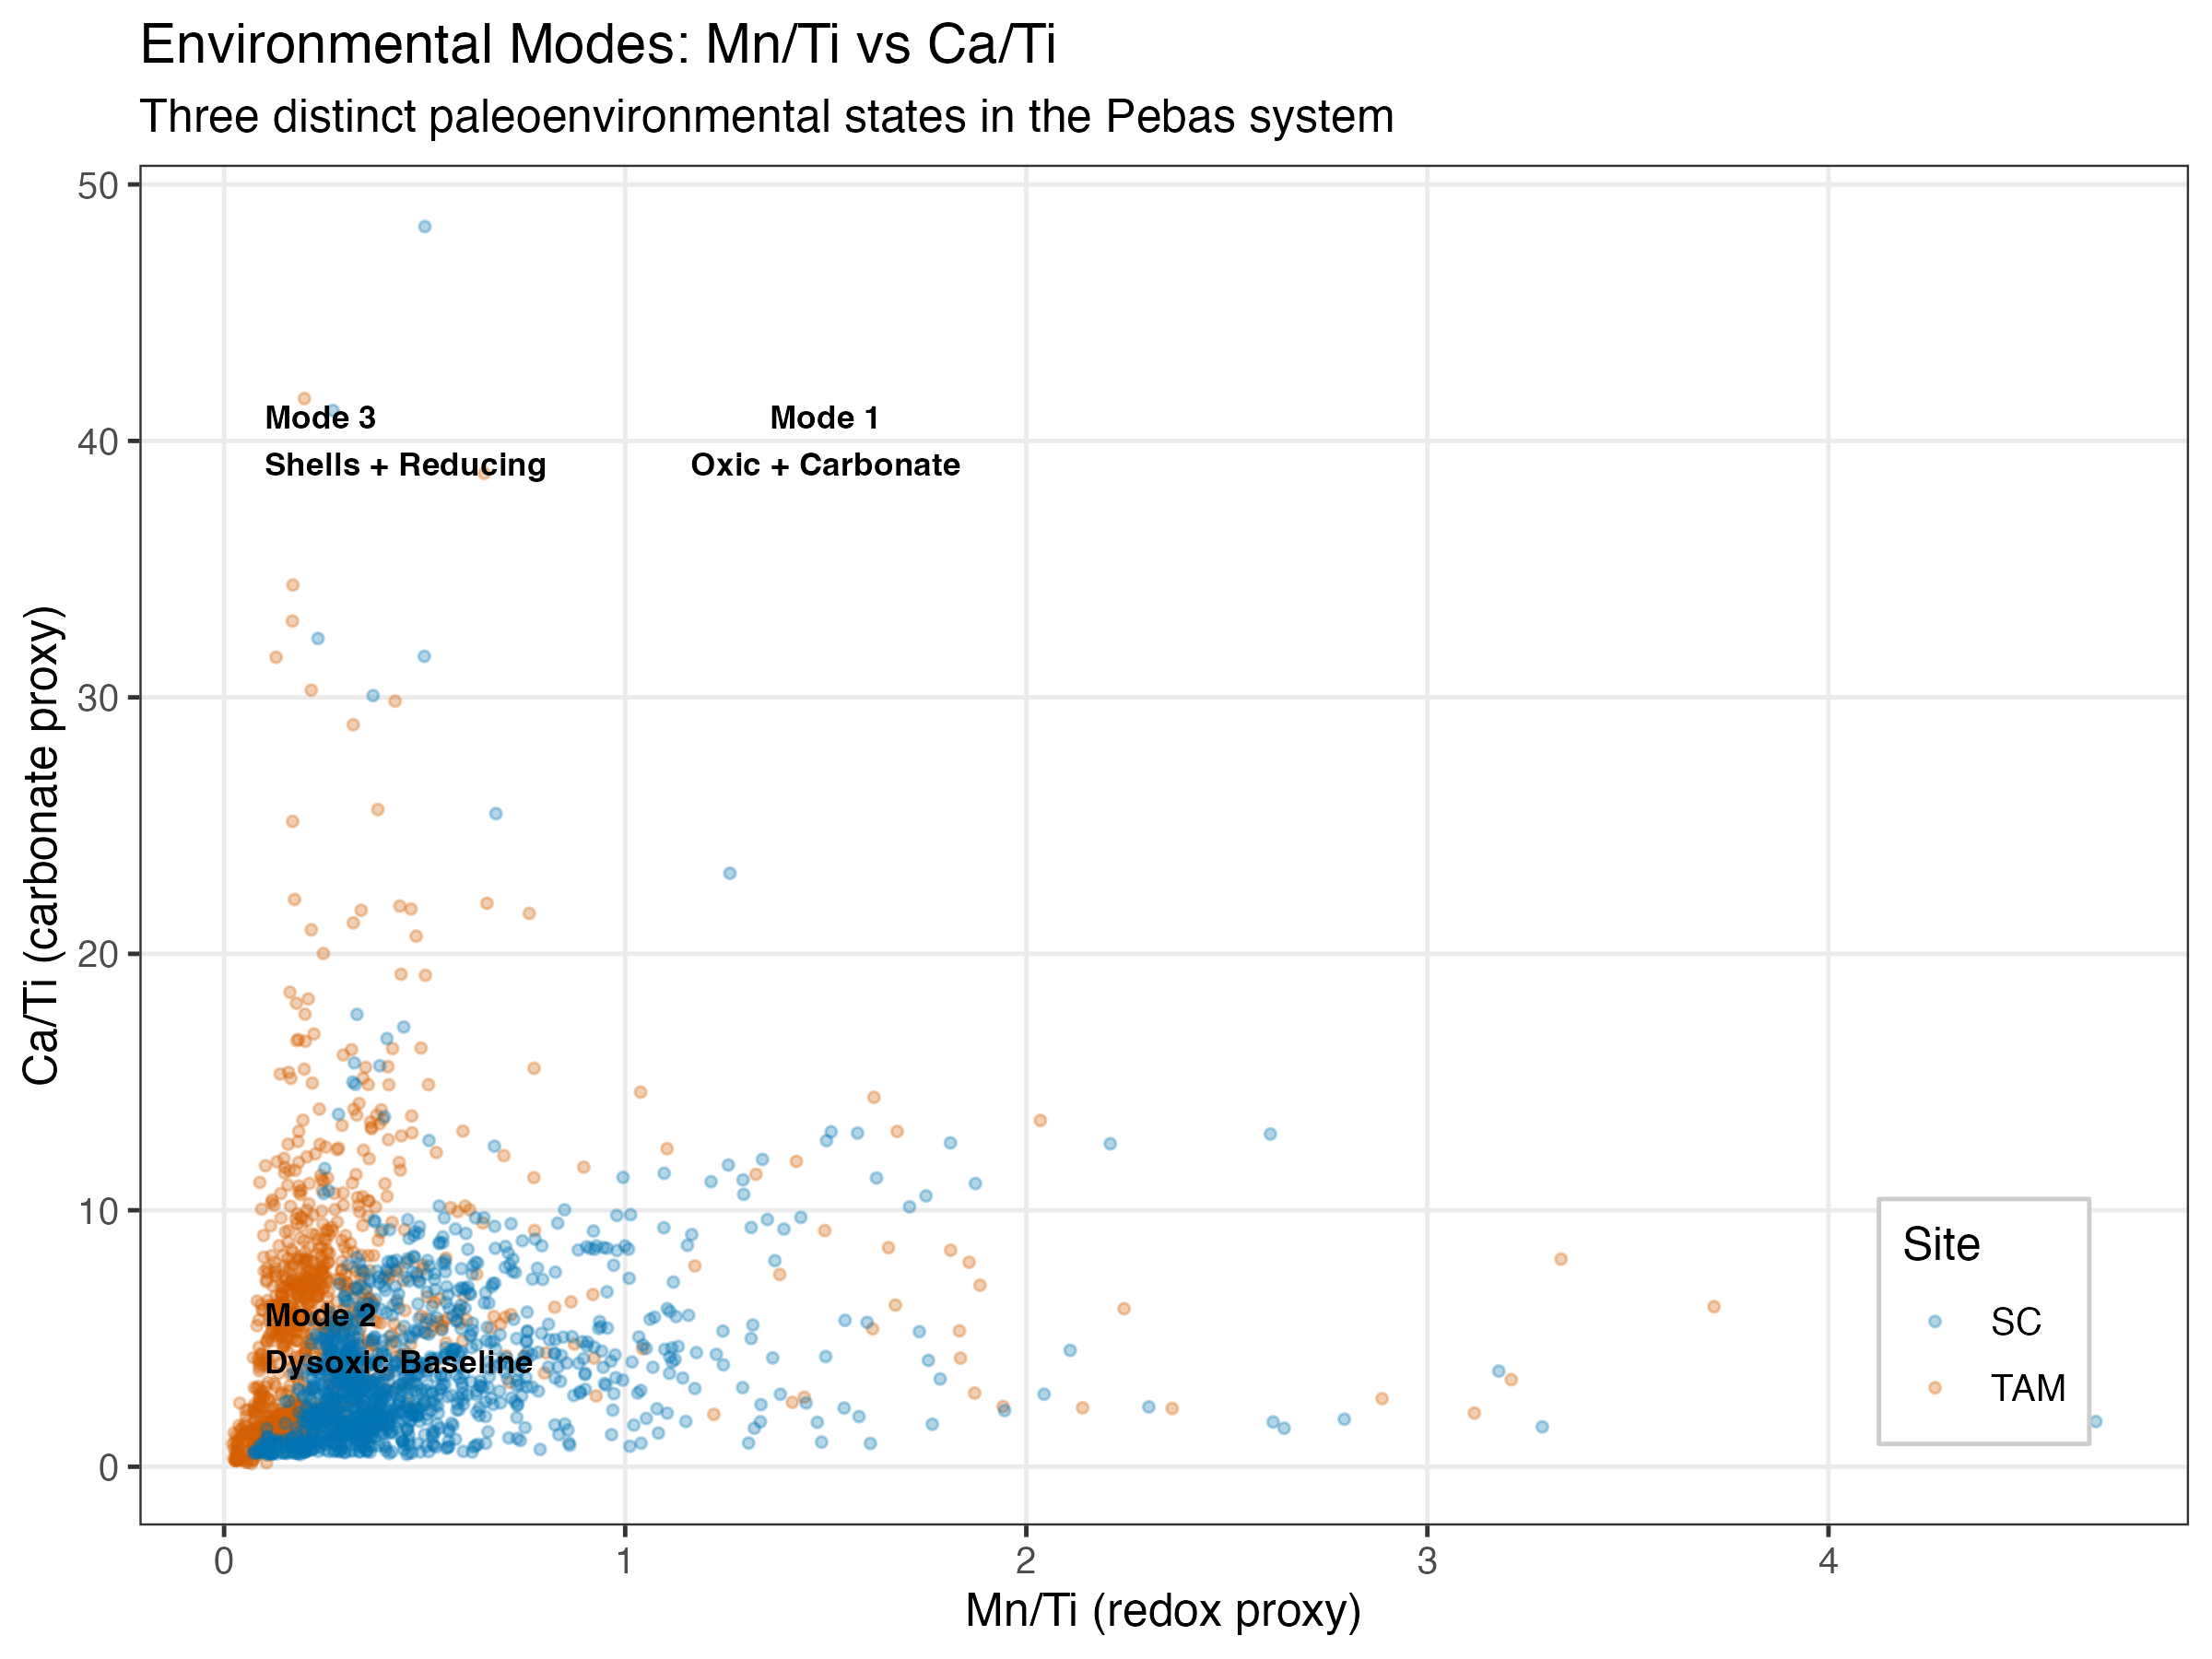
\includegraphics[width=0.9\textwidth]{../output/figures/temporal_overlap/fig7_environmental_modes.png}
    \caption{Environmental modes from Mn/Ti vs Ca/Ti crossplot. Three distinct states emerge, each with different preservation potential and ecological character.}
    \label{fig:modes}
\end{figure}

\begin{table}[H]
\centering
\caption{Environmental modes and their paleontological significance}
\begin{tabular}{lllll}
\toprule
Mode & Mn/Ti & Ca/Ti & Environment & Preservation \\
\midrule
\textbf{Dysoxic Baseline} & Low & Low-Med & Stratified, anoxic & Excellent (articulated) \\
\textbf{Oxic-Carbonate} & High & High & Ventilated, productive & Moderate (shells) \\
\textbf{Shell Accumulation} & Low & High & Transport into dysoxic & Good (concentrated) \\
\bottomrule
\end{tabular}
\end{table}

\subsection{Depositional Model}

\begin{table}[H]
\centering
\caption{Depositional settings in the Pebas mega-wetland}
\begin{tabular}{lllll}
\toprule
Setting & Site & Characteristics & XRF Signature & Fossils \\
\midrule
Distal lacustrine & TAM & Stratified, dysoxic & Low Mn/Ti, high Ca/Ti & Articulated vertebrates \\
Fluvio-lacustrine & SC & Ventilated, dynamic & High Mn/Ti, variable & Mollusc-rich beds \\
\bottomrule
\end{tabular}
\end{table}

\subsection{XRF as Preservation Predictor}

\begin{table}[H]
\centering
\caption{XRF-based preservation prediction}
\begin{tabular}{llll}
\toprule
Mn/Ti Value & Oxygen Regime & Preservation Quality & Expected Fossils \\
\midrule
$<$ 0.10 & Strongly anoxic & Exceptional & Articulated skeletons, soft tissues \\
0.10--0.20 & Dysoxic & Very Good & Complete shells, associated bones \\
0.20--0.40 & Suboxic & Moderate & Disarticulated but identifiable \\
$>$ 0.40 & Oxic & Poor & Scattered, abraded fragments \\
\bottomrule
\end{tabular}
\end{table}

%==============================================================================
\section{Conclusions}
%==============================================================================

\begin{enumerate}
    \item \textbf{Top of cores comparison} reveals that TAM (youngest sections, $\sim$12.9 Ma) maintains its dysoxic character while SC (youngest sections, $\sim$13.3 Ma) shows higher oxygenation---fundamental site differences persist through time.

    \item \textbf{Temporal overlap analysis} (13.275--13.446 Ma) confirms that the TAM-SC contrast reflects \textbf{spatial heterogeneity} within the Pebas mega-wetland, not simply temporal evolution.

    \item \textbf{Case studies} demonstrate that XRF proxies successfully identify:
    \begin{itemize}
        \item Sustained dysoxia favorable for exceptional preservation (TAM-3A-4-5CDE-A)
        \item Shell-rich horizons indicating productivity events (SC-3AB-4ABCD-A)
        \item Environmental transitions and high-frequency variability
    \end{itemize}

    \item The \textbf{Pebas mega-wetland} supported two coexisting environmental modes: a stratified, dysoxic lacustrine setting (TAM) and a ventilated, dynamic fluvio-lacustrine setting (SC), separated by only 30 km.

    \item \textbf{XRF-based taphonomy} can predict preservation quality: Mn/Ti $<$ 0.2 indicates the ``taphonomic sweet spot'' for articulated fossil preservation.
\end{enumerate}

%==============================================================================
\section{Quick Reference}
%==============================================================================

\begin{table}[H]
\centering
\caption{Key numbers}
\begin{tabular}{ll}
\toprule
\multicolumn{2}{c}{\textbf{Chronology}} \\
\midrule
TAM age range & 12.935--13.446 Ma \\
SC age range & 13.275--14.298 Ma \\
Overlap & 171 kyr (13.275--13.446 Ma) \\
\midrule
\multicolumn{2}{c}{\textbf{Key Results}} \\
\midrule
TAM Mn/Ti median & 0.18 (dysoxic) \\
SC Mn/Ti median & 0.37 (suboxic) \\
Site O$_2$ difference & 2.1$\times$ \\
\bottomrule
\end{tabular}
\end{table}

%==============================================================================
\section*{References}
%==============================================================================

\begin{itemize}[noitemsep]
    \item Hoorn, C. et al. (2010). The development of the Amazonian mega-wetland. In: Amazonia: Landscape and Species Evolution.
    \item Kaandorp, R.J.G. et al. (2005). Ecological implications from geochemical records of Miocene Western Amazonian bivalves.
    \item Salas-Gismondi, R. et al. (2015). A Miocene hyperdiverse crocodylian community reveals peculiar trophic dynamics in proto-Amazonian mega-wetlands.
    \item Wesselingh, F.P. (2006). Evolutionary ecology of the Pachydontinae.
\end{itemize}

\end{document}
